% ----------------------------------------------------------- % 
\chapter{GCN-based models for cancer driver gene prediction}
\label{sec:gcn_model}


In this chapter, we provide a deeper examination of the prediction of CDGs using the GCN algorithm, which showed the most promising performance in the experimental comparison presented in Chapter~\ref{sec:results:comparative_evaluation}. We detail the investigation of the best set of hyperparameters for the three smaller PPI networks and the three larger PPI networks. We also report the performance of GCN models trained with each of the six PPI networks using a common independent test set. Finally, we compare the predictive performance of the models trained on the collected PPI networks with those trained on the UNION PPI network defined in our work (as explained in Section~\ref{sec:materials_methods:ppinets}) and ensemble-based approaches (as detailed in Section~\ref{sec:ensemble_training}).



\section{Experiments setup}
\label{sec:gcn_model:setup}

In this series of experiments, we aimed to optimize the hyperparameters of the GCN algorithm to try to achieve higher predictive performance. Specifically, we conducted hyperparameter optimization for each of the PPI networks collected from the literature, namely HPRD, MULTINET, IREF, CPDB, PCNET, and STRING.

To ensure a fair comparison between models for the same set of test genes, we randomly split the main dataset into training and test sets considering only positively and negatively labeled genes common to all PPI networks for the test set. With this, we generated a fixed test set used in these experiments. We then used 5-fold cross-validation in the training set to evaluate the performance during hyperparameter optimization. All models were trained using the multi-omics data and centrality measures as node features.

After hyperparameter optimization, we trained a final model using the best hyperparameter configuration and the complete training set, and applied it to predict the label for the independent test set and for the unlabeled nodes present in each PPI network. The first dataset allowed us to evaluate the final performance of the model, while the second dataset aimed to suggest potential candidate driver genes for further investigation.

In the following sections, we describe the creation of the independent test set used in these experiments and the hyperparameter optimization strategy adopted.




\subsection{Creation of an independent test set} 
\label{sec:independent_testset}


To create the independent test set for this series of experiments, we searched for genes present in all six PPI networks collected. We identified a set of 8,068 genes, which represents 41.2\% of the total number of genes included in all networks (\ie the union of genes among all PPI networks). Taking as reference the smallest PPI network, which is the HPRD network, we estimated the number of genes to withhold for the test considering an 80:20 ratio for training and test sets. We found that about 1,134 labeled genes should be reserved as a test set to follow this proportion of data split for the smallest network. 

Then, we randomly selected 1,134 labeled genes among those that are common to all six PPI networks in a stratified fashion, generating an independent test set with 159 driver genes (\ie positive examples) and 975 passenger genes (\ie negative examples). This test set was fixed during our experiments in the sense that it was the same test set used for all PPI networks. The strategy adopted causes the proportion of the test set to vary among PPI networks, as shown in Figure \ref{fig:split_traintest}. For example, the test set represents only 8.5\% of the total number of genes in the PCNET network. However, reserving 20\% of labeled data for the test set based on the number of genes comprised in the largest network would cause a considerable restriction of data for training the models from small PPI networks such as the HPRD. Therefore, in this chapter, all the results reported for the independent test set will refer to exactly the same set of 159 driver genes and 975 passenger genes.


\begin{figure*}[!th]
    \centering
      \caption{Proportion of training and test sets for all PPI networks considering a fixed set of labeled genes for testing.}
    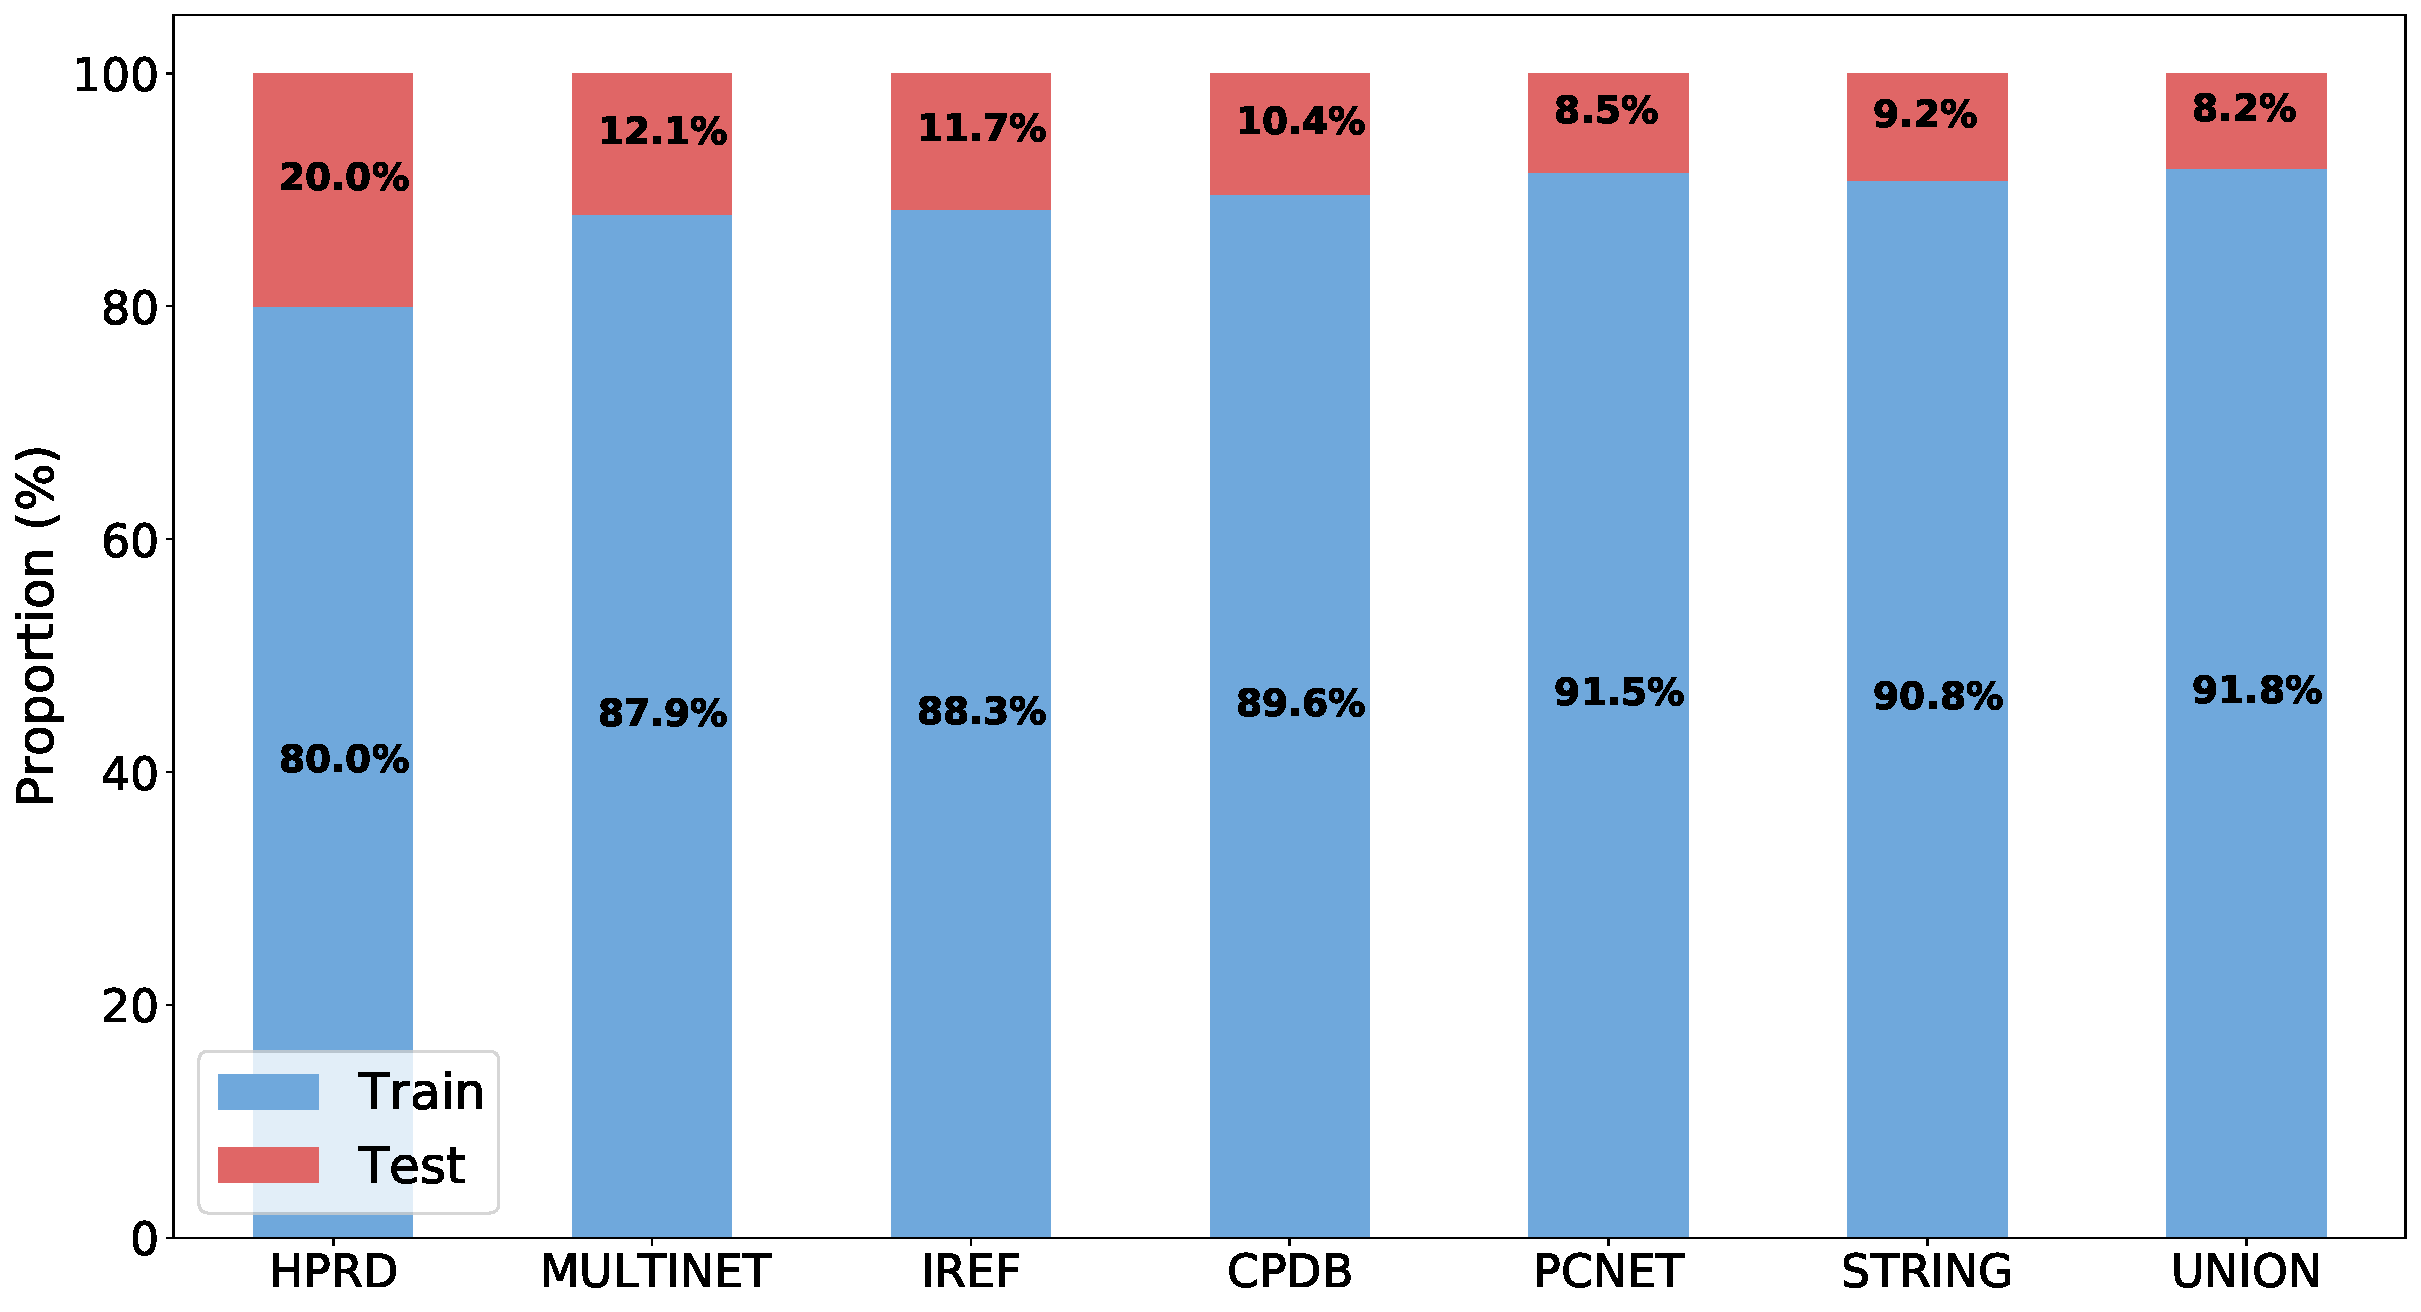
\includegraphics[width=0.93\textwidth]{images/results/split_traintest.pdf}
    \legend{Source: Prepared by the author}
    \label{fig:split_traintest}
\end{figure*}

\subsection{Strategy for hyperparameter optimization}
Table \ref{tab:hyperparameters_range} lists the hyperparameters that were chosen for the investigation conducted in this chapter and the values that were initially included in the grid search, selected based on the recommendations discussed in Chapter~\ref{sec:materials_methods}. 



\begin{table}[!h]
\centering
\caption{Hyperparameters evaluated for GCN training with HPRD, MULTINET, and IREF networks \label{tab:hyperparameters_range}}
\begin{tabular}{ll}
\hline
\multicolumn{1}{c}{Hyperparameter}   & \multicolumn{1}{c}{Values tested} \\ \hline
Number of layers                      & 2                                    \\
Number of neurons/units on each layer & 64; 128; 256                         \\
Activation function                   & ELU; ReLU                            \\
Dropout                               & 0.001; 0.01; 0.1                     \\
Learning rate                         & 0.00001; 0.0001; 0.001               \\
Number of epochs                      & 500                                  \\
Focal loss (gamma)                    & 0; 0.5; 1; 2                         \\
Focal loss (alpha)                    & 0.25; 0.50; 0.75; 0.90               \\ \hline
\end{tabular}
\end{table}

The training process for the GCN algorithm involves a total of 864 combinations of hyperparameters related to the learning algorithm and to the focal loss function. Evaluating all these combinations can be computationally expensive due to the complexity of the PPI network, especially for the three largest PPI networks, resulting in long execution times. Therefore, we adopted a strategy to simplify the search grid in these cases. 
First, we evaluated all the 864 combinations of hyperparameters for the three smallest PPI networks, namely HPRD, MULTINET, and IREF, which have less than 140,000 edges. Based on the results obtained for this first round of experiments, we carried out a performance impact analysis of hyperparameter values. 

For this analysis, we defined a set of thresholds for AUC-PR performance and counted the number of hyperparameter combinations that produced results higher than the threshold, for each cutoff defined. The thresholds \{0.2, 0.4\} were used for the three PPI networks, but the set was extended with higher threshold values that were closer to the maximum AUC-PR performance obtained for each PPI network analyzed. The higher the performance threshold applied, the fewer the number of hyperparameter combinations attached to the training process that achieved that minimum performance mark. The intention was to extract a fine-grained analysis of the relation of hyperparameters values and AUC-PR performance for top-performing models.

Then, we analyzed the most frequent values of hyperparameters for each performance threshold. We investigated, for instance, the existence of specific hyperparameter values that were never related to high performance, or, in contrast, that were very frequent among the models with outstanding results. We used the findings of this analysis to prune or to adjust the grid of hyperparameter values for the second round of experiments involving the three largest PPI networks. 

This approach was implemented in response to the intricacy of GNN techniques. Specifically, the execution time of a training epoch for a small network, such as HPRD, is typically measured in milliseconds, whereas larger networks, such as STRING, require approximately 8 seconds to complete a single epoch, on average. Furthermore, even the GCN algorithm, which is the most expeditious of the three GNN algorithms examined in the preceding chapter, still necessitates a nontrivial amount of computational time.

\section{Results}

\subsection{Hyperparameter optimization for the three smallest PPI networks}


The hyperparameter values used for the HPRD, MULTINET, and IREF networks were presented in Table \ref{tab:hyperparameters_range}. As previously mentioned, a total of 864 configurations were assessed for the smallest PPI networks. The average performance of models in the validation set (\ie the independent folds in the 5-fold CV) was analyzed for each hyperparameter configuration. 
Observing the general panorama of this evaluation, as summarized in Figure~\ref{fig:val_lollipop_hprd} for the HPRD network, we can note that there are hyperparameters combinations that were clearly not promising in terms of the achieved performance, while others stood out in this aspect. In other words, there is a discernible trend in higher and lower performance according to the hyperparameters configuration adopted. This trend was also observed for the analysis of the results obtained for the two other smallest networks, MULTINET and IREF, as shown in the appendix (Figure~\ref{fig:val_lollipop_multinet_iref}).


\begin{figure*}[!th]
    \centering
      \caption{Performance analysis of all hyperparameter combinations for the HPRD network.}
    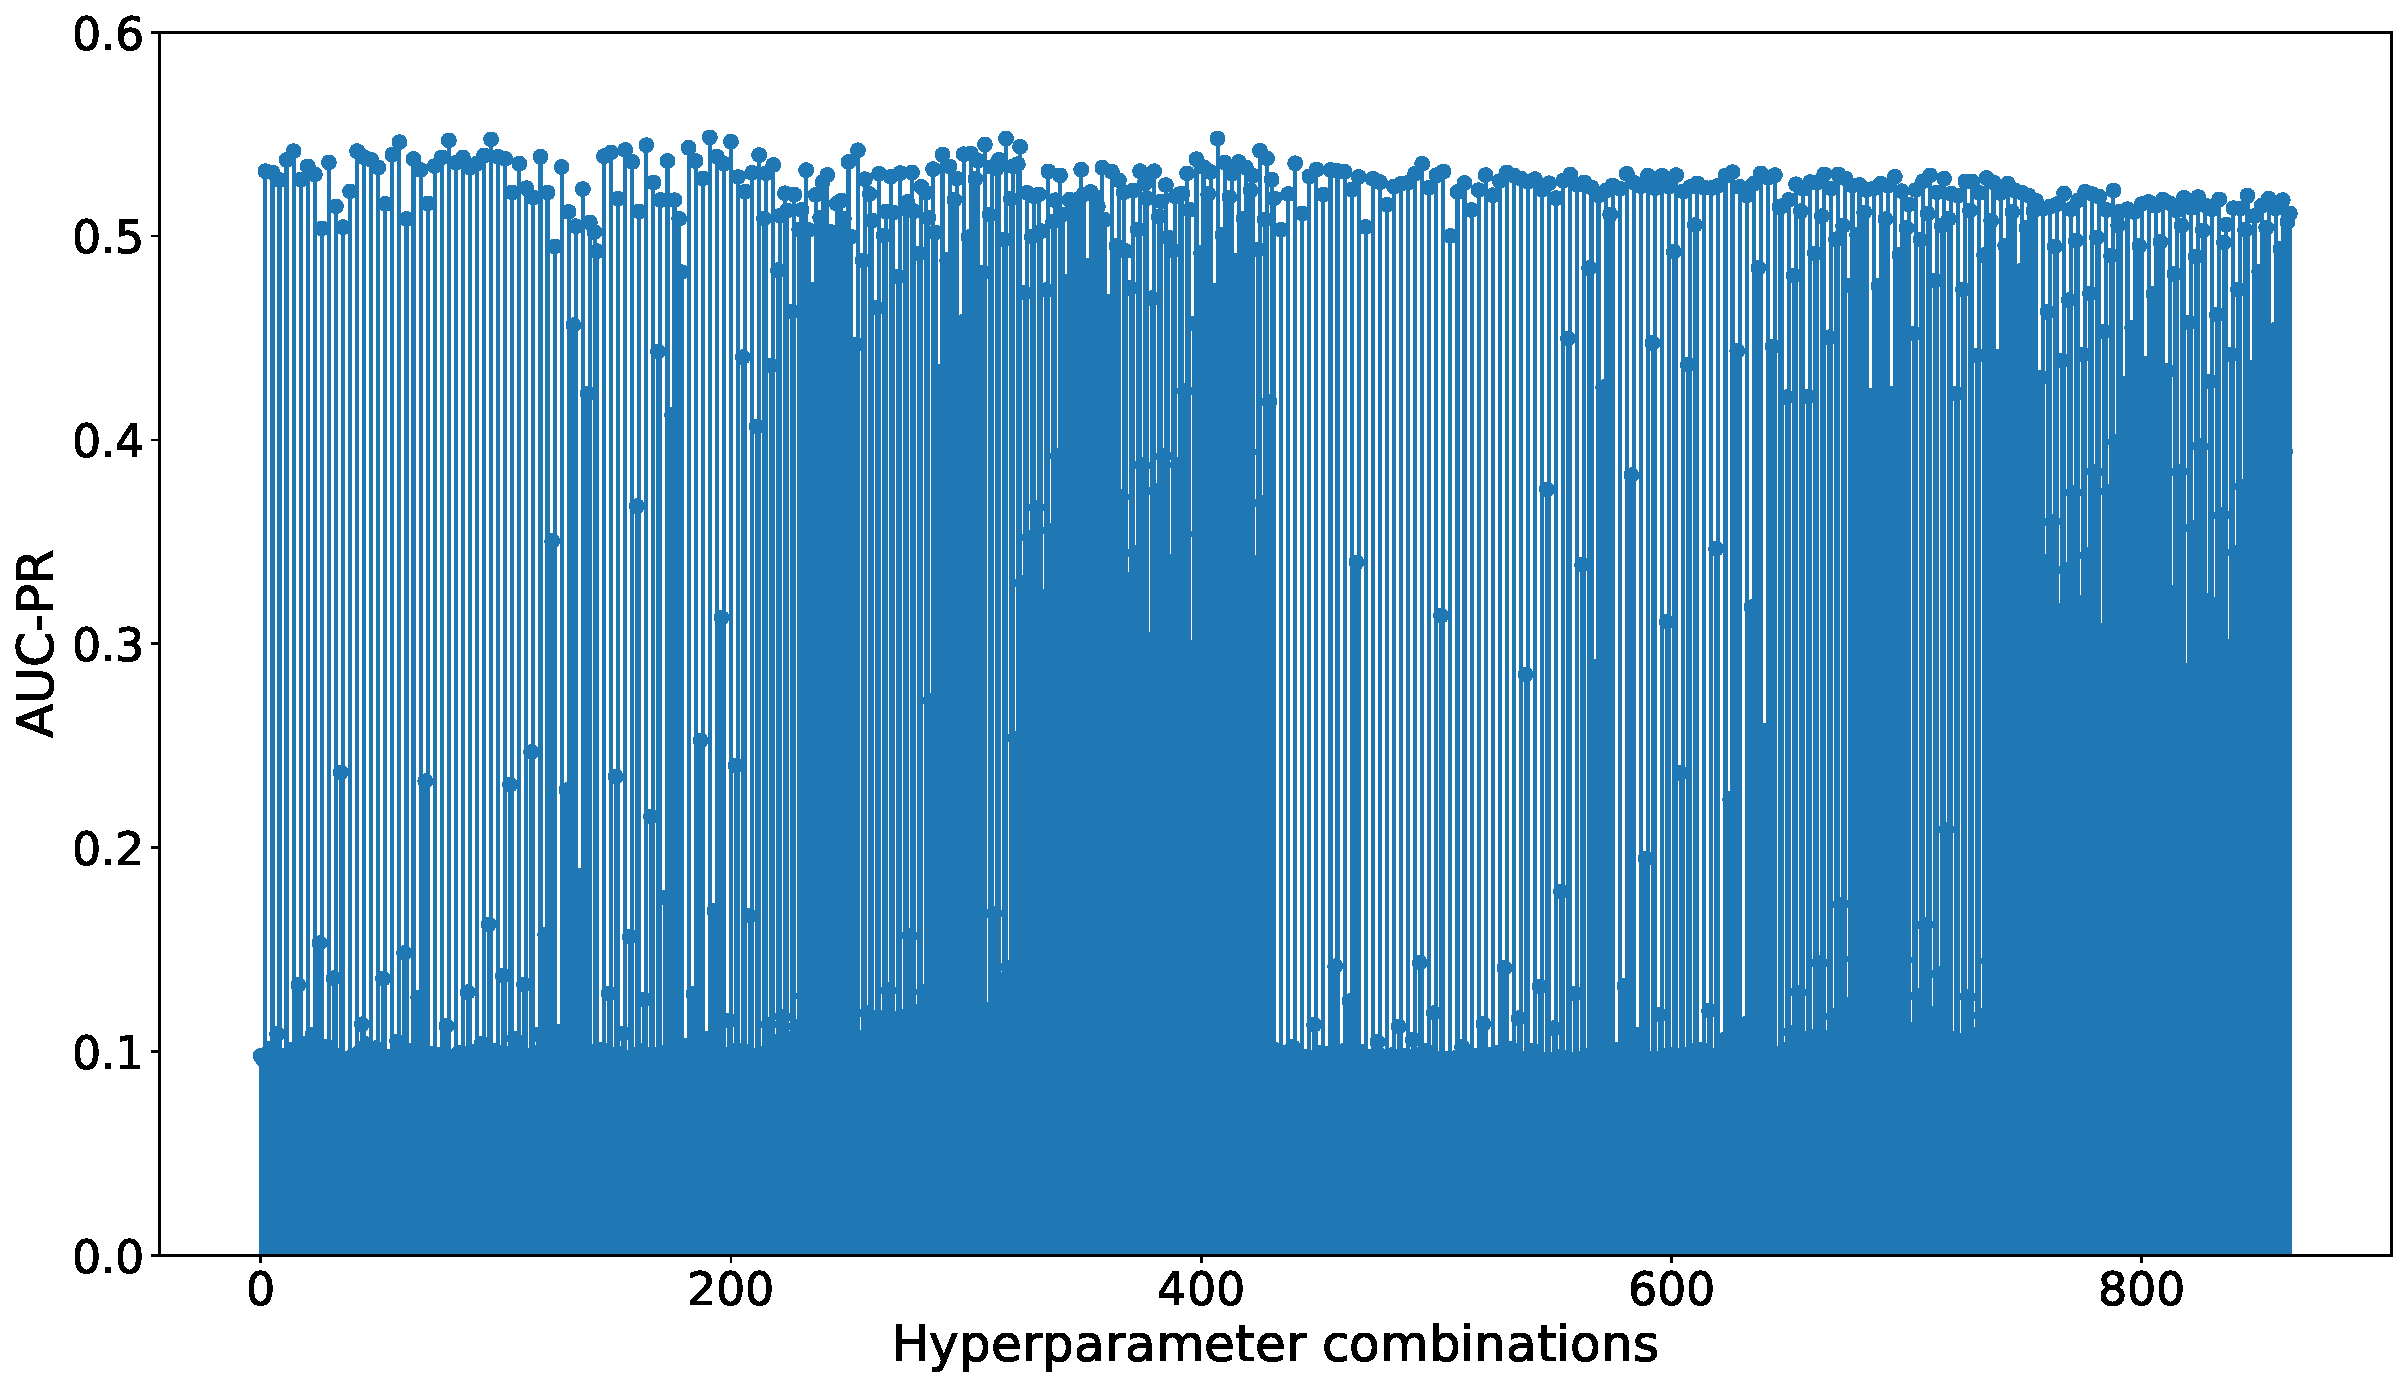
\includegraphics[width=\textwidth]{images/results/val_lollipop_hprd.pdf}
    \legend{Source: Prepared by the author}
    \label{fig:val_lollipop_hprd}
\end{figure*}




\begin{table}[!ht]
\centering
\caption{Occurrence frequency of hyperparameters values for the models trained with the HPRD network using AUC-PR threshold of 0.53. A total of 97 combinations met the criteria. \label{tab:analise_parametros}}
\begin{tabular}{llllll}
\hline
\multicolumn{2}{c}{Activation function}       & \multicolumn{2}{c}{Alpha ($\alpha$)}                        & \multicolumn{2}{c}{Gamma ($\gamma$)}                      \\ \hline
ReLU & {\color[HTML]{333333} \textbf{84.5\%}} & 0.25    & {\color[HTML]{333333} \textbf{36.0\%}} & 0     & {\color[HTML]{333333} 22.6\%}          \\
ELU  & 15.4\%                                 & 0.5     & 22.6\%                                 & 0.5   & {\color[HTML]{333333} \textbf{27.8\%}} \\
     &                                        & 0.75    & {\color[HTML]{333333} 23.7\%}          & 1     & {\color[HTML]{333333} \textbf{27.8\%}} \\
     &                                        & 0.9     & 17.5\%                                 & 2     & 21.6\%                                 \\ \hline
\multicolumn{2}{c}{Number of neurons}         & \multicolumn{2}{c}{Learning rate}                & \multicolumn{2}{c}{Dropout}                    \\ \hline
64   & {\color[HTML]{333333} \textbf{39.1\%}} & 0.00001 & 0.0\%                                  & 0.001 & 24.7\%                                 \\
128  & 30.9\%                                 & 0.0001  & 9.2\%                                  & 0.01  & 27.8\%                                 \\
256  & 29.8\%                                 & 0.001   & {\color[HTML]{333333} \textbf{90.7\%}} & 0.1   & {\color[HTML]{333333} \textbf{47.4\%}} \\ \hline
\end{tabular}
\end{table}


To illustrate how we conducted the impact analysis of hyperparameter combinations, we show in the  Table~\ref{tab:analise_parametros} the results for the HPRD network considering an AUC-PR performance threshold of 0.53. Filtering the results by this threshold yielded a total of 97 hyperparameter combinations\footnote{For comparison purpose, when considering the HPRD PPI network, using the threshold of AUC-PR > 0.2 we obtained 556 combinations of hyperparameter values, using the threshold AUC-PR > 0.4 we obtained 457 combinations, and using the threshold AUC-PR > 0.5 we obtained 350 combinations.}.  We observed, for instance, that higher learning rates occurred more frequently, to the extent that the lowest learning rate (\ie 0.00001) employed was never selected among the 97 combinations that met the AUC-PR threshold applied. 
In summary, higher learning rates seem to produce more effective classification results. Some hyperparameters are still inconclusive as to their impact on the predictive power, especially because their impact varies according to the network analyzed. 

Only two hyperparameters had clear and similar patterns across the three PPI networks that were significant for planning the next round of hyperameraters optimization: the learning rate and the activation function.  Thus, for the largest PPI networks, it was possible to reduce the number of parameter combinations by approximately one-third just by adjusting two hyperparameters, the activation function, for which we only maintained the ``ReLU'' function, and the learning rate. For the learning rate, we removed the two smallest values from the original grid, and used 0.001 and 0.005, where the latter was a new value included for training the largest PPI networks.


Figure \ref{fig:val_boxplot1} shows the performance variation for the top five combinations of hyperparameters in the experiments with (a) HPRD, (b) MULTINET, and (c) IREF networks. The validation performance in the last training epoch in each of the five folds is observed and used to report these results, with the white dot representing the mean. Additionally, the best hyperparameter combination according to the average performance in the validation sets is highlighted in green. We observed that the median performance is around 0.60 for HPRD, and around 0.5 for MULTINET and IREF. Although the median performance if very close among the top 5 configurations, some specific hyperparameter combinations lead to larger variations in performance or to the occurrence of outliers.


\begin{figure*}[!ht]
\centering

\caption{Five best combinations of parameters for (a) HPRD, (b) MULTINET and (c) IREF.}

   \subfloat[HPRD \label{val_boxplot_hprd}]{%
      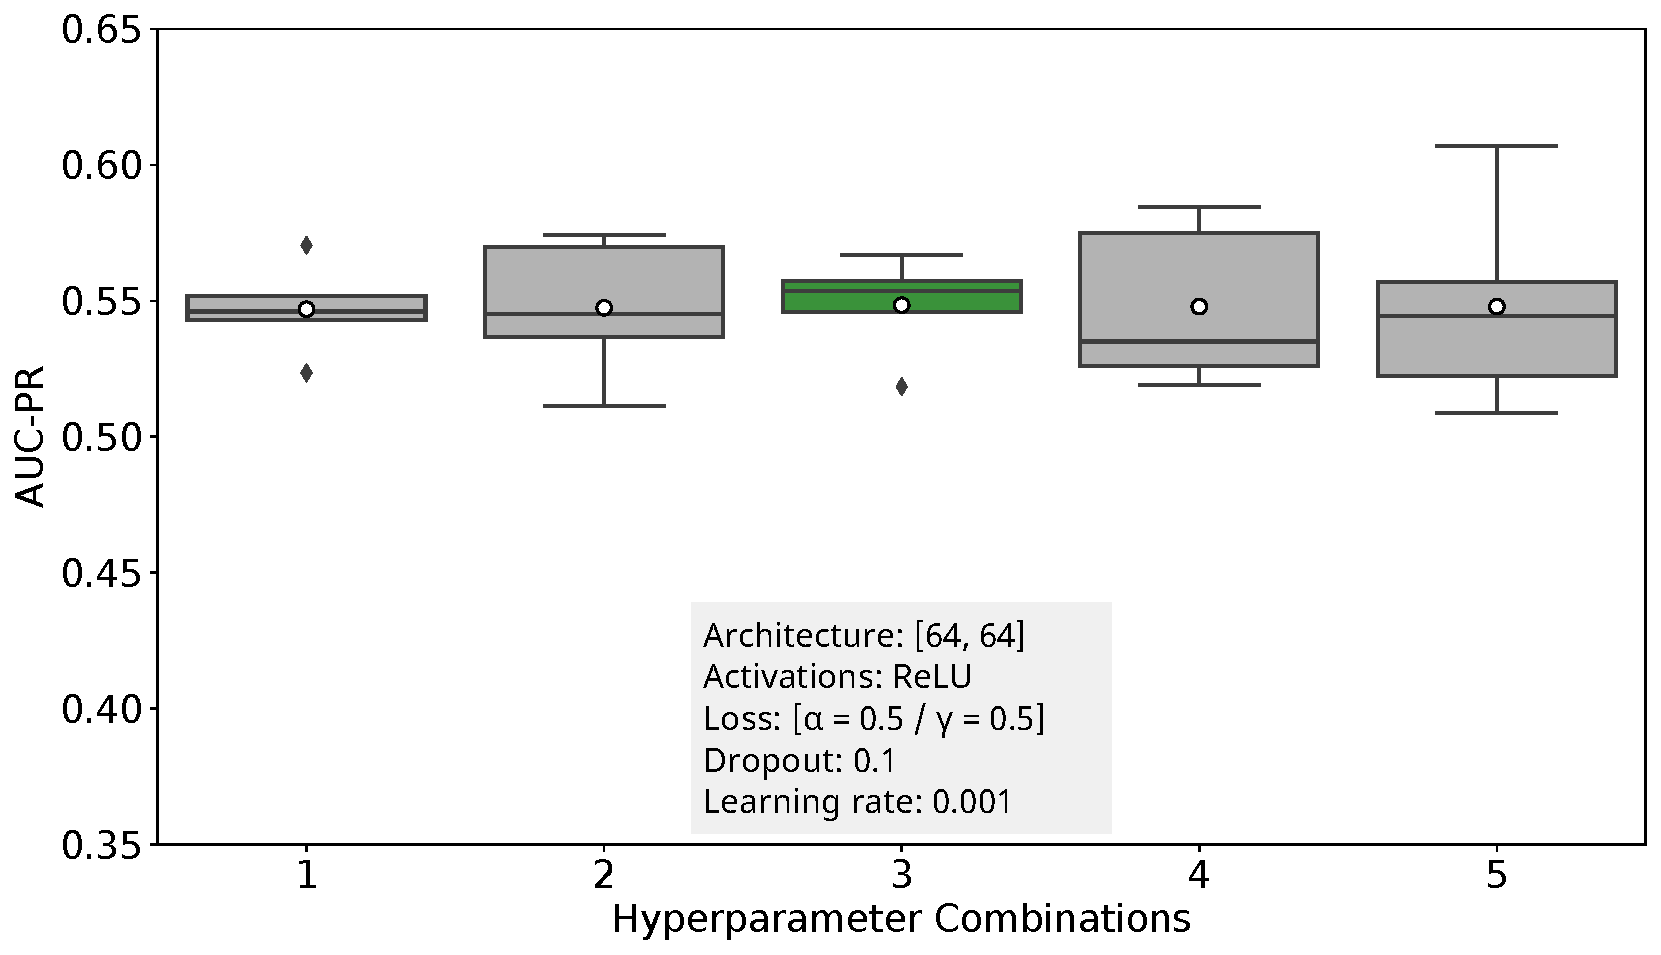
\includegraphics[width=0.72\textwidth]{images/results/val_boxplot_hprd.pdf}}
\hspace{0em}
   \subfloat[MULTINET \label{val_boxplot_multinet} ]{%
      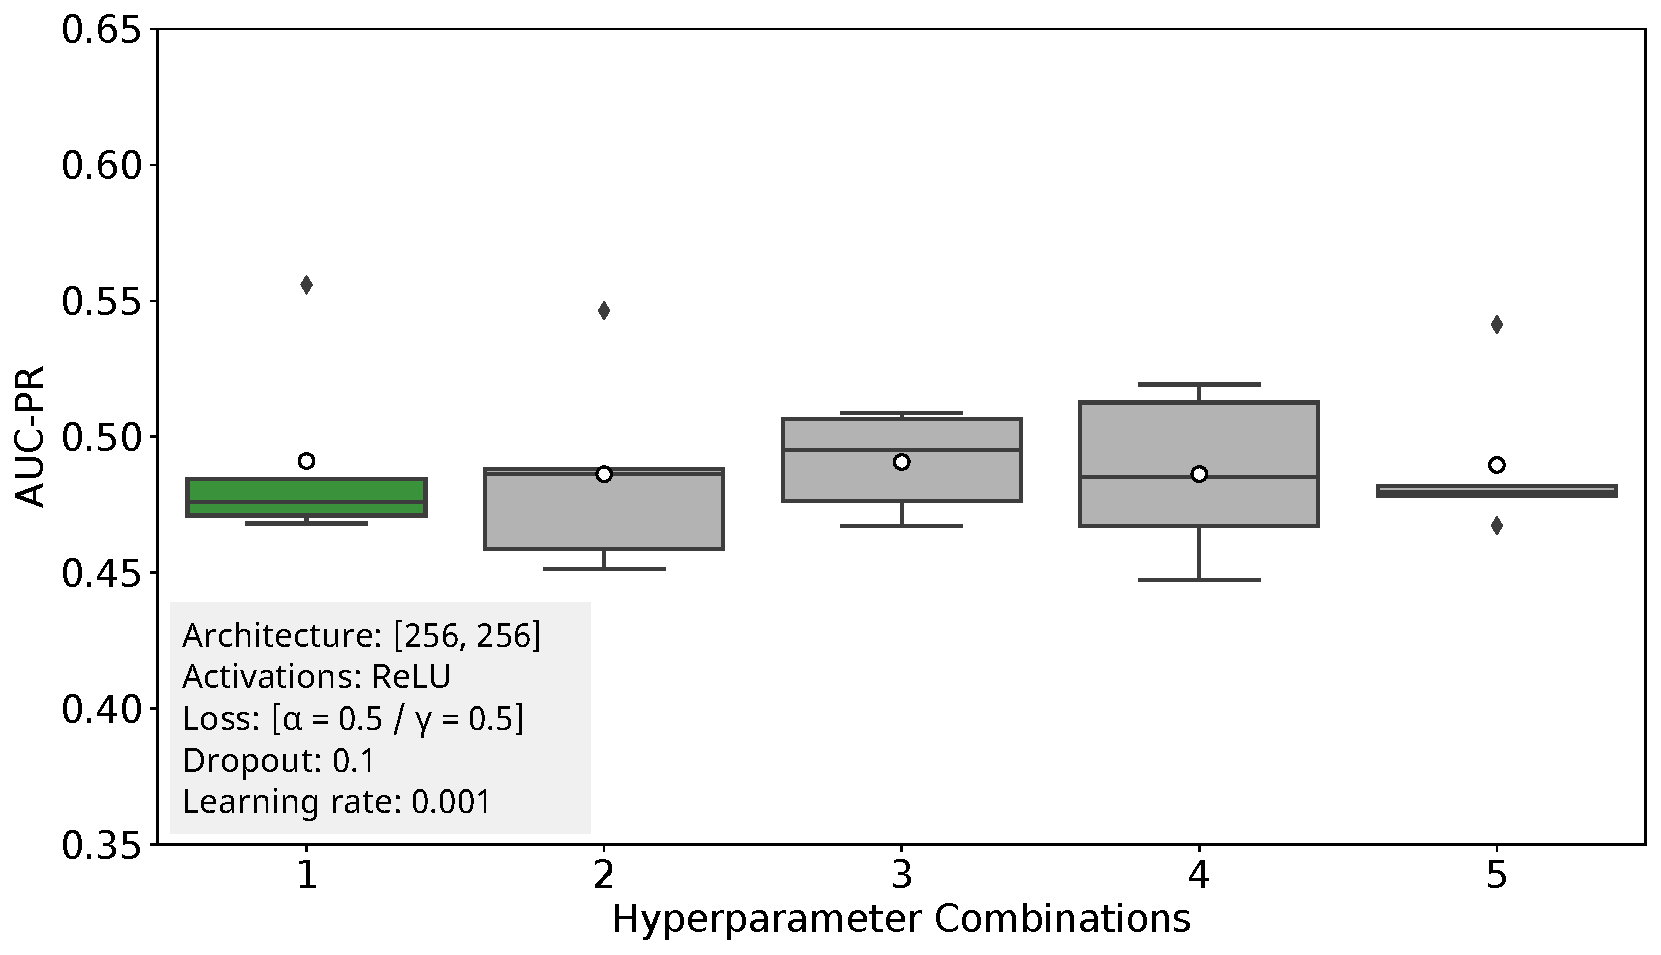
\includegraphics[width=0.72\textwidth]{images/results/val_boxplot_multinet.pdf}}
\hspace{0em}
   \subfloat[IREF \label{val_boxplot_iref}]{%
      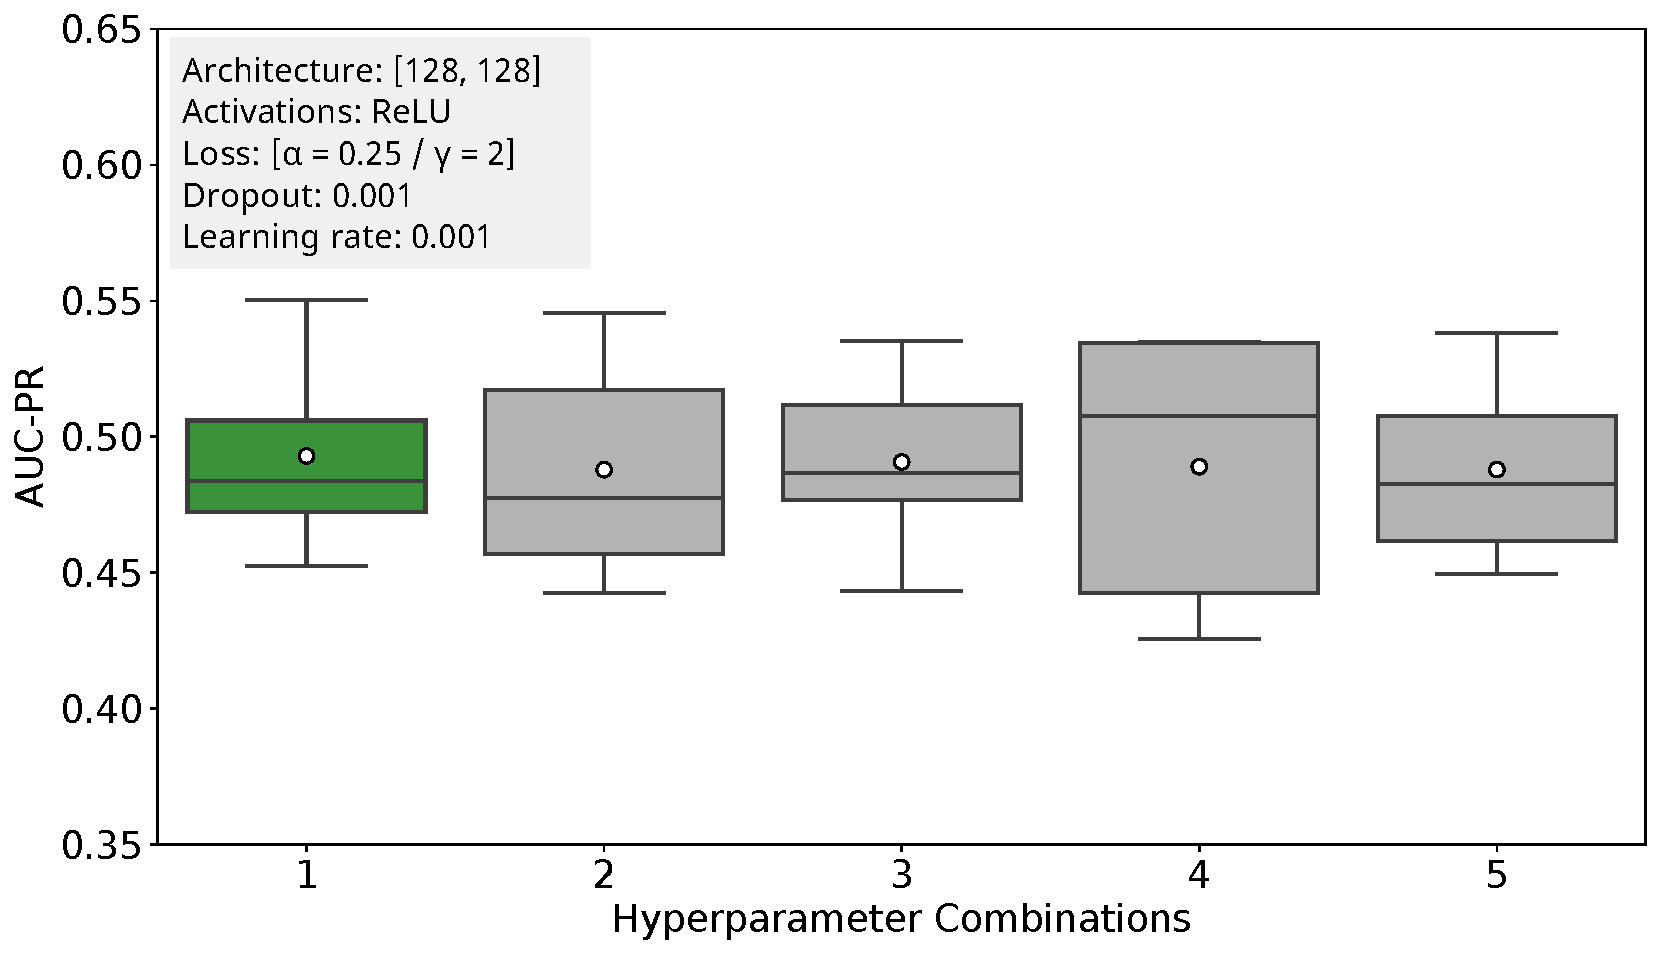
\includegraphics[width=0.72\textwidth]{images/results/val_boxplot_iref.pdf}}\\

\label{fig:val_boxplot1}
\end{figure*}




\subsection{Hyperparameter optimization for the three largest PPI networks}

The CPDB, PCNET, and STRING networks belong to the group of largest PPI networks, having more than 1.5 million edges. Processing these networks requires significant computational power and longer execution time for each experiment. Therefore, to address this issue, we modified the grid of hyperparameter values based on the results described in the previous section. The modified grid is shown in Table~\ref{tab:hyperparameters_range_filt} and it reduces the number of hyperparameter combinations to a total of 288 possible combinations.



\begin{table}[!h]
\centering
\caption{Hyperparameters evaluated for GCN training with CPDB, PCNET, and STRING networks \label{tab:hyperparameters_range_filt}}
\begin{tabular}{ll}
\hline
\multicolumn{1}{c}{Hyperparameter}   & \multicolumn{1}{c}{Parameter Ranges} \\ \hline
Number of layers                      & 2                                    \\
Number of neurons/units on each layer & 64; 128; 256                         \\
Activation function                   & ReLU                            \\
Dropout                               & 0.001; 0.01; 0.1                     \\
Learning rate                         & 0.001; 0.005               \\
Number of epochs                      & 500                                  \\
Focal loss (gamma)                    & 0; 0.5; 1; 2                         \\
Focal loss (alpha)                    & 0.25; 0.50; 0.75; 0.90               \\ \hline
\end{tabular}
\end{table}


\begin{figure*}[!hb]
    \centering
      \caption{Performance analysis of all hyperparameter combinations for the STRING network.}
    
\includegraphics[width=\textwidth]{images/results/val_lollipop_string.pdf}
    \legend{Source: Made by the author}
    \label{fig:val_lollipop_string}
\end{figure*}

Again, based on an overview of the results for the STRING network (Figure~\ref{fig:val_lollipop_string}), we also noticed that the AUC-PR values varied according to the hyperparameter values used. However, the amplitude of changes was lower than those observed in the experiments for the smallest networks. In fact, most of the models trained using the STRING network achieved an AUC-PR value close to 0.5, with similar results obtained for the other PPI networks explored in this round of experiments (Figure \ref{fig:val_lollipop_cpdb_pcnet}).



\begin{figure*}[!ht]
\centering
\caption{Five best combinations of parameters for (a) CPDB, (b) PCNET and (c) STRING.}

   \subfloat[CPDB \label{val_boxplot_cpdb}]{%
      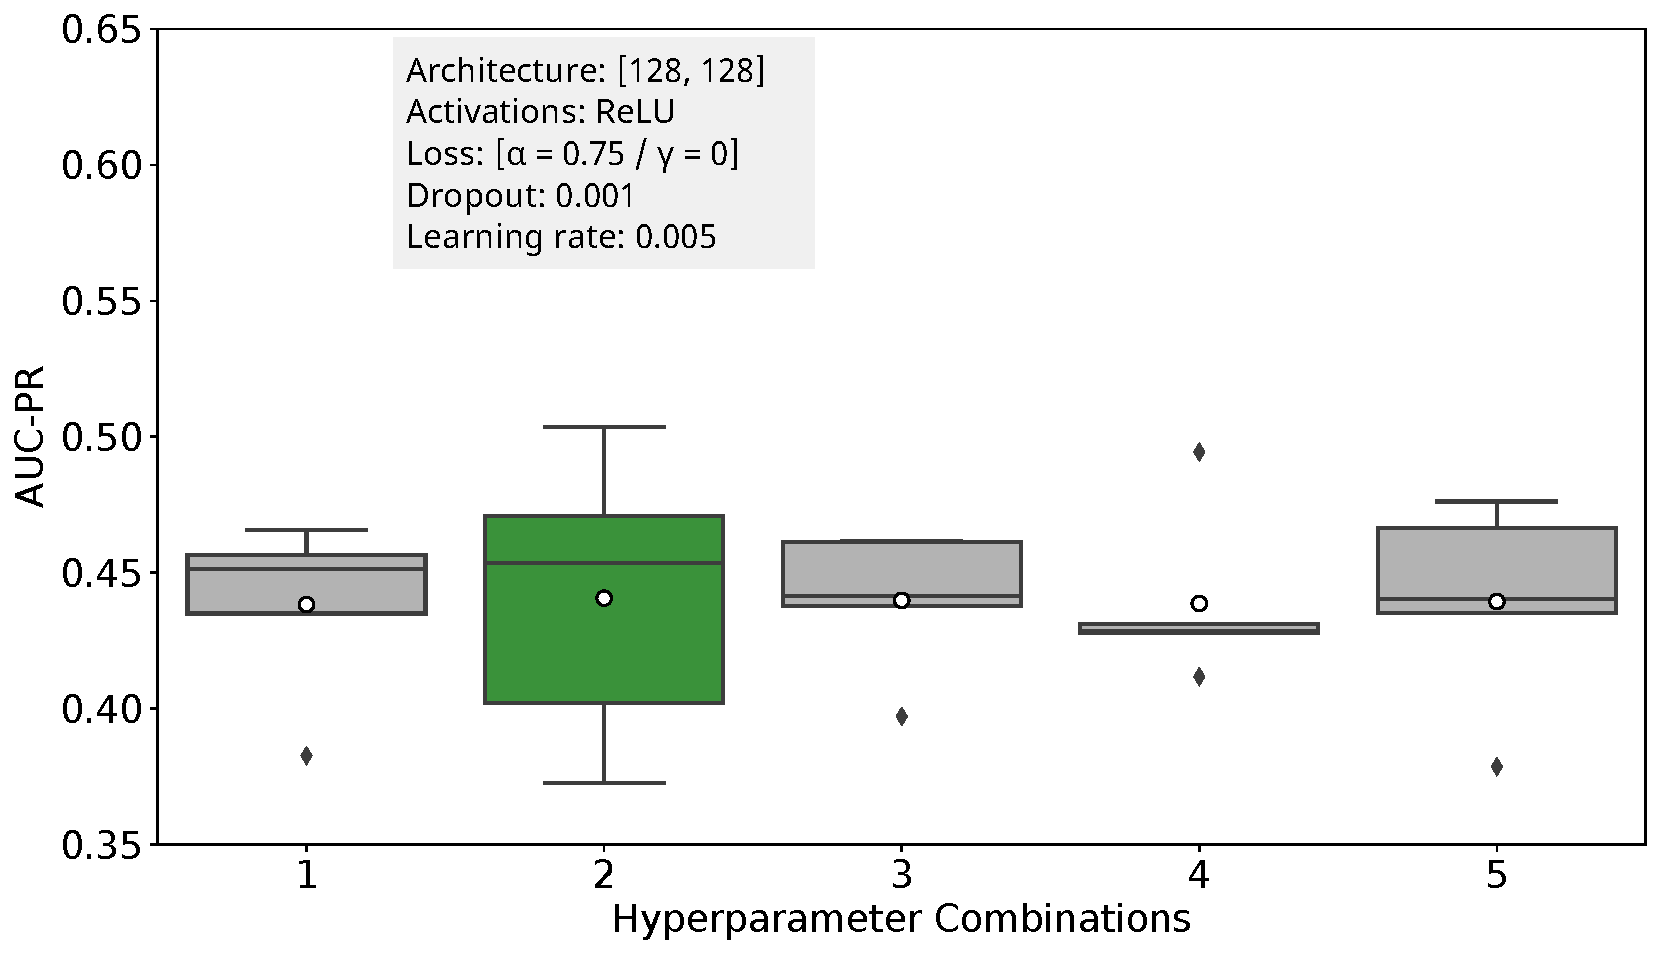
\includegraphics[width=0.72\textwidth]{images/results/val_boxplot_cpdb.pdf}}
\hspace{0em}
   \subfloat[PCNET \label{val_boxplot_pcnet} ]{%
      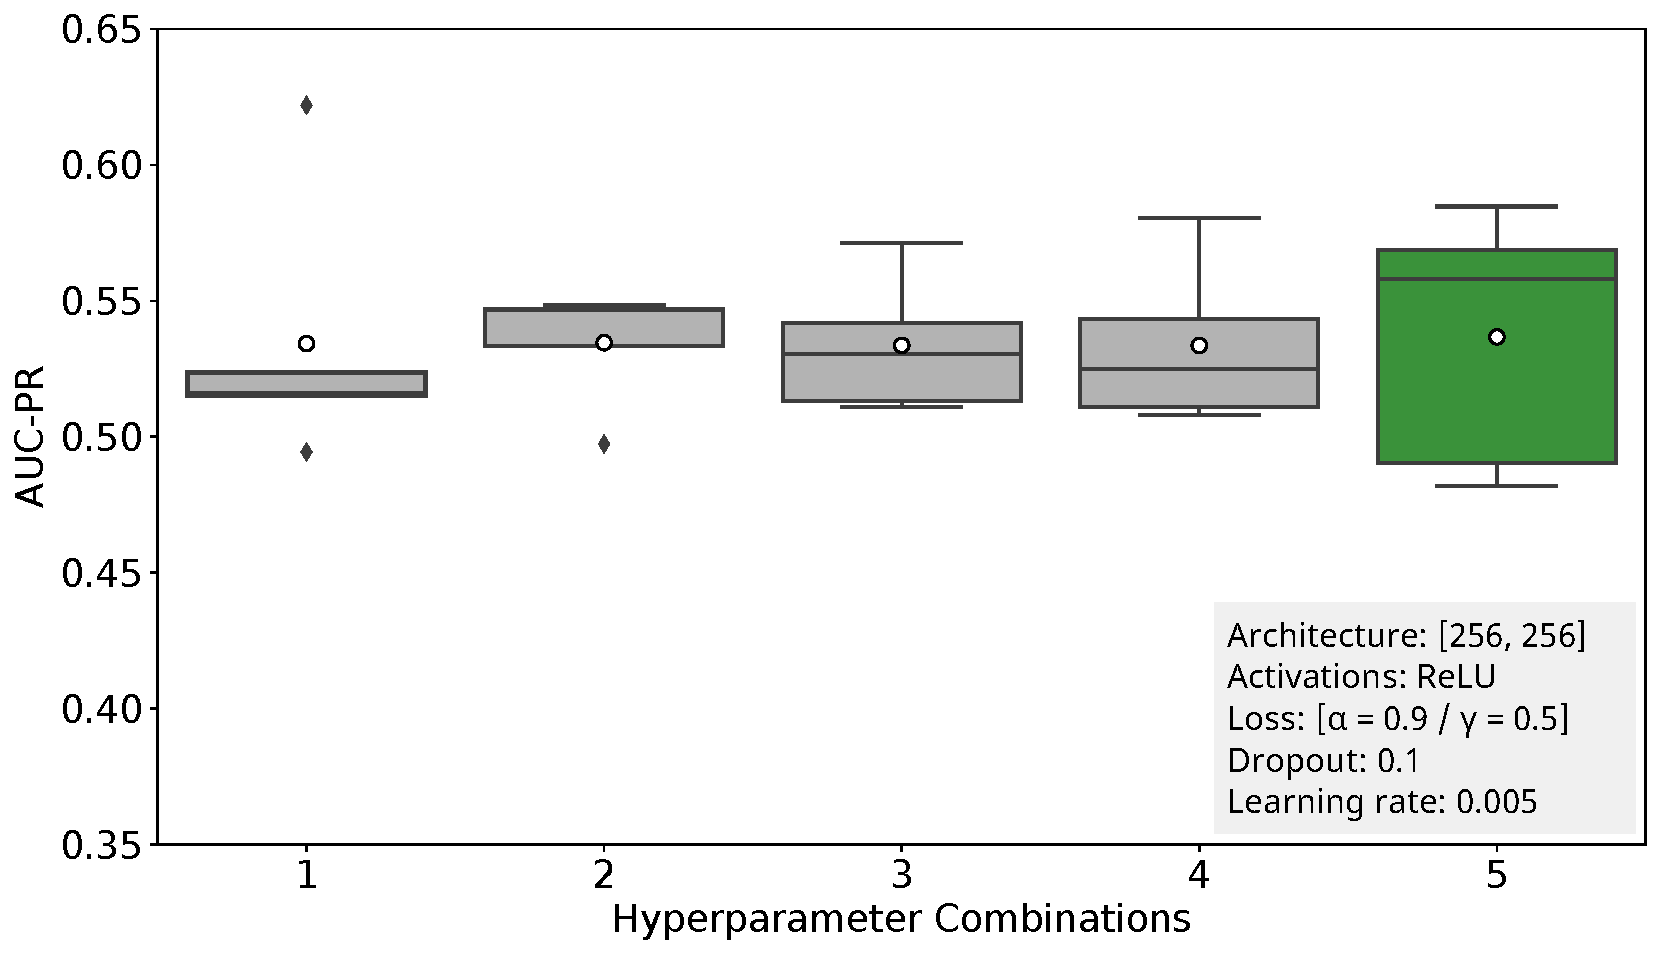
\includegraphics[width=0.72\textwidth]{images/results/val_boxplot_pcnet.pdf}}
\hspace{0em}
   \subfloat[STRING \label{val_boxplot_string}]{%
      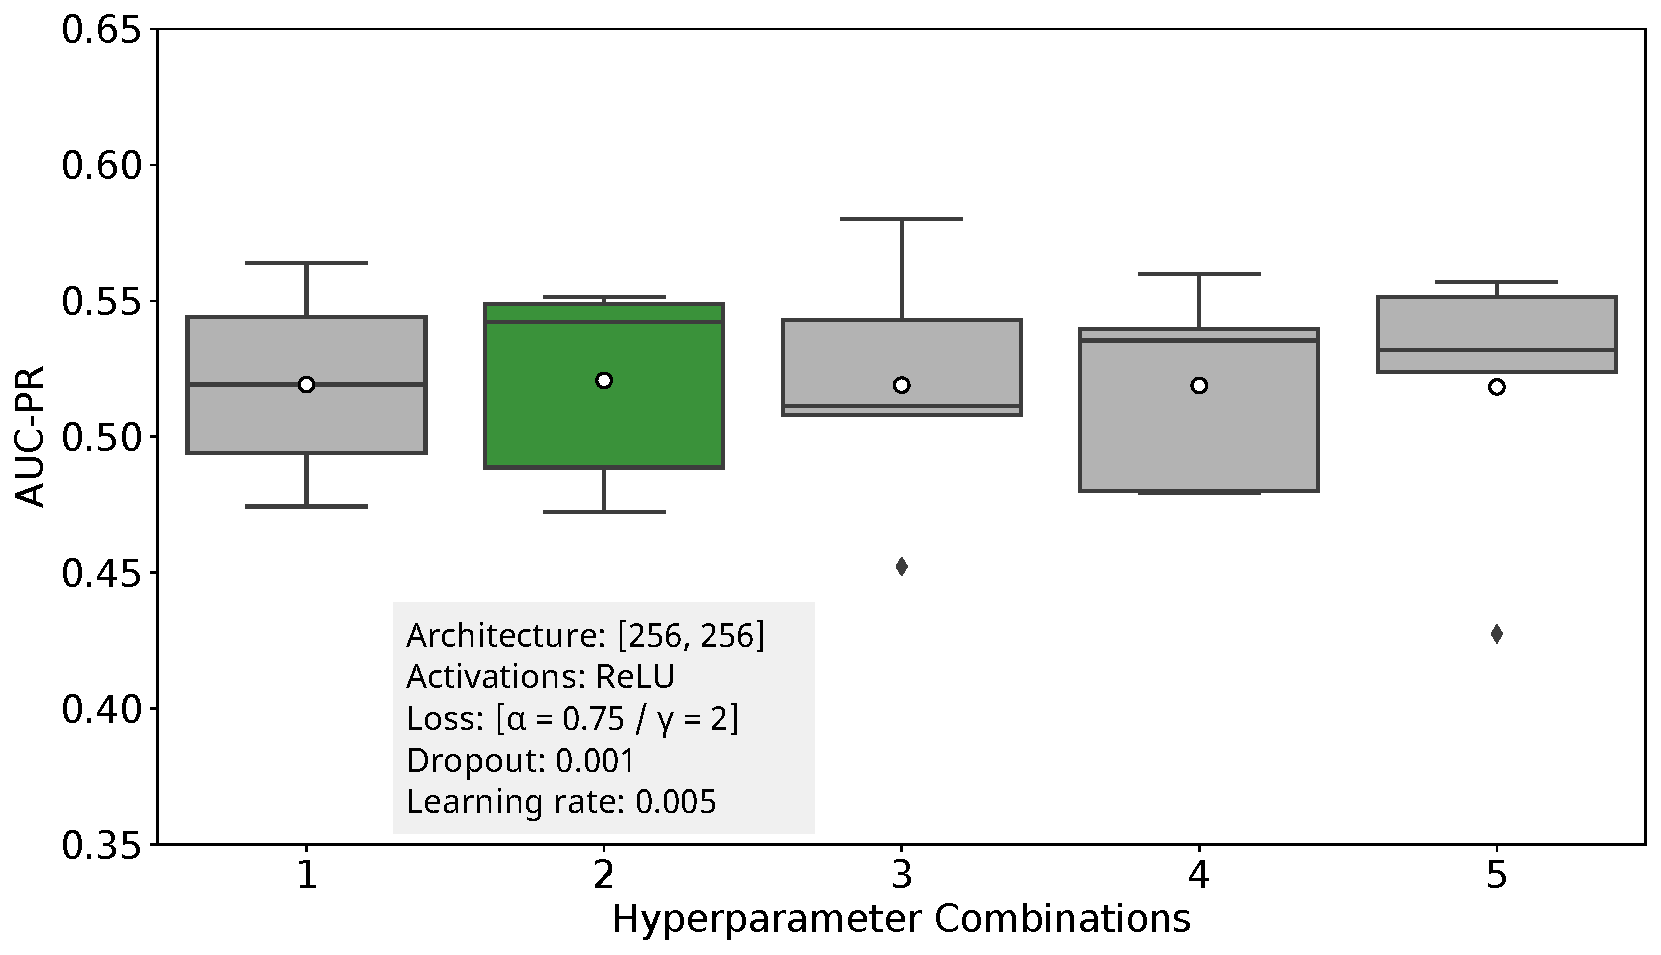
\includegraphics[width=0.72\textwidth]{images/results/val_boxplot_string.pdf}}\\
\label{fig:val_boxplot2}
\end{figure*}


One interesting finding is that the PPI largest networks did not necessarily outperform all the smallest networks, although, theoretically, they carry out more information about the molecular aspects of genetic interactions. The best performance for validation data was obtained with PCNET (\ie AUC-PR = 0.5367). Figure \ref{fig:val_boxplot2} shows the five best combinations of hyperparameters for each of the largest networks analyzed. Although this average performance of around 0.5 seems low, it shows the complexity that the studied algorithms face in dealing with class imbalance, even when applying mitigation strategies. Therefore, higher values for metrics such as accuracy and AUC-ROC may not represent the prediction goal we aim to achieve.

Leveraging the results of the hyperparameters optimization for all the PPI networks, the next sections will present the results for model training and evaluation using the fixed independent test set defined in Section~\ref{sec:independent_testset}.




\subsection{Predictive performance of individual GCN-based models for the test set}

Following hyperparameters optimization, the best hyperparameter values obtained for each PPI network were applied to train GCN-based models for the prediction of CDGs as explained in Section~\ref{sec:gcn_model:setup}. These values are summarized in Table~\ref{tab:top_hiperparametros}. 
We investigate the performance of the models during training and validation through the learning curves, but we focus the analysis on the performance for the fixed test set described in Section~\ref{sec:independent_testset}.





\begin{table}[!h]
\centering
\caption{Best hyperparameter configuration found for each PPI network. \label{tab:top_hiperparametros}}
\begin{tabular}{lcccccc}
\hline
              & HPRD   & MULTINET & IREF     & CPDB     & PCNET    & STRING   \\ \hline
Layer sizes   & 64; 64 & 256; 256 & 128; 128 & 128; 128 & 256; 256 & 256; 256 \\
Activation    & ReLU   & ReLU     & ReLU     & ReLU     & ReLU     & ReLU     \\
Dropout       & 0.1    & 0.1      & 0.001    & 0.001    & 0.1      & 0.001    \\
Learning rate & 0.001  & 0.001    & 0.001    & 0.005    & 0.005    & 0.005    \\ 
Loss (alpha)  & 0.5    & 0.5      & 0.25     & 0.75     & 0.9      & 0.75     \\
Loss (gamma)  & 0.5    & 0.5      & 2        & 0        & 0.5      & 2        \\
\hline
\end{tabular}
\end{table}



We selected three PPI networks that obtained the best results, regardless of their dimension, to present the training and validation performance in this section. Figure \ref{fig:aucpr_roc_best3} presents the main metrics observed in the experiments (\ie AUC-PR and AUC-ROC) for MULTINET, PCNET, and STRING. The other PPI networks are analyzed in the Appendix, Figure~\ref{fig:aucpr_roc_worse3}. Furthermore, because the focal loss function has its own hyperparameters and each PPI network has been optimized with different combinations of the focal loss hyperparameters, the loss curves for these experiments are also provided in the Appendix (Figure \ref{fig:loss_allnetworks}).


\begin{figure*}[!ht]
\centering

\caption{AUC-PR and AUC-ROC performance for GCN models trained with (a) MULTINET, (b) PCNET, and (c) STRING networks.}

   \subfloat[MULTINET \label{aucpr_roc_multinet}]{%
      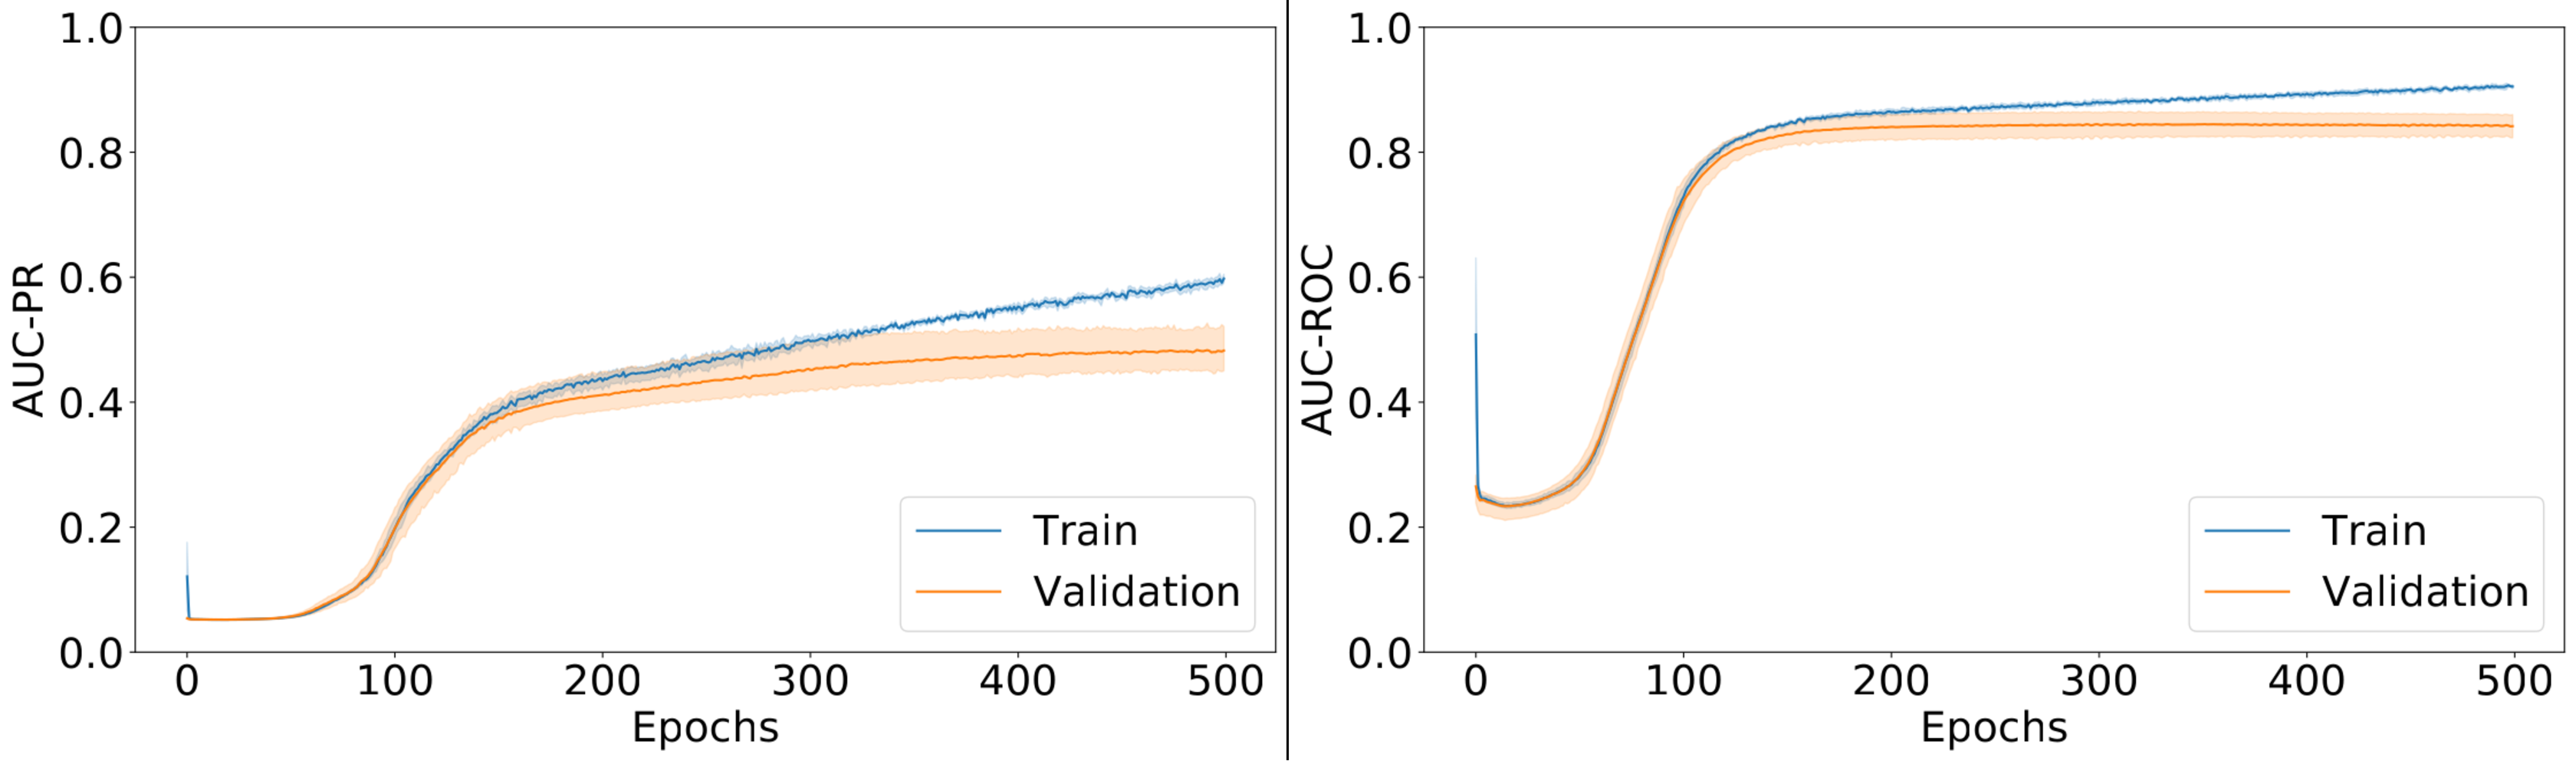
\includegraphics[width=\textwidth]{images/results/aucpr_roc_multinet.pdf}}
\hspace{\fill}
   \subfloat[PCNET \label{aucpr_roc_pcnet} ]{%
      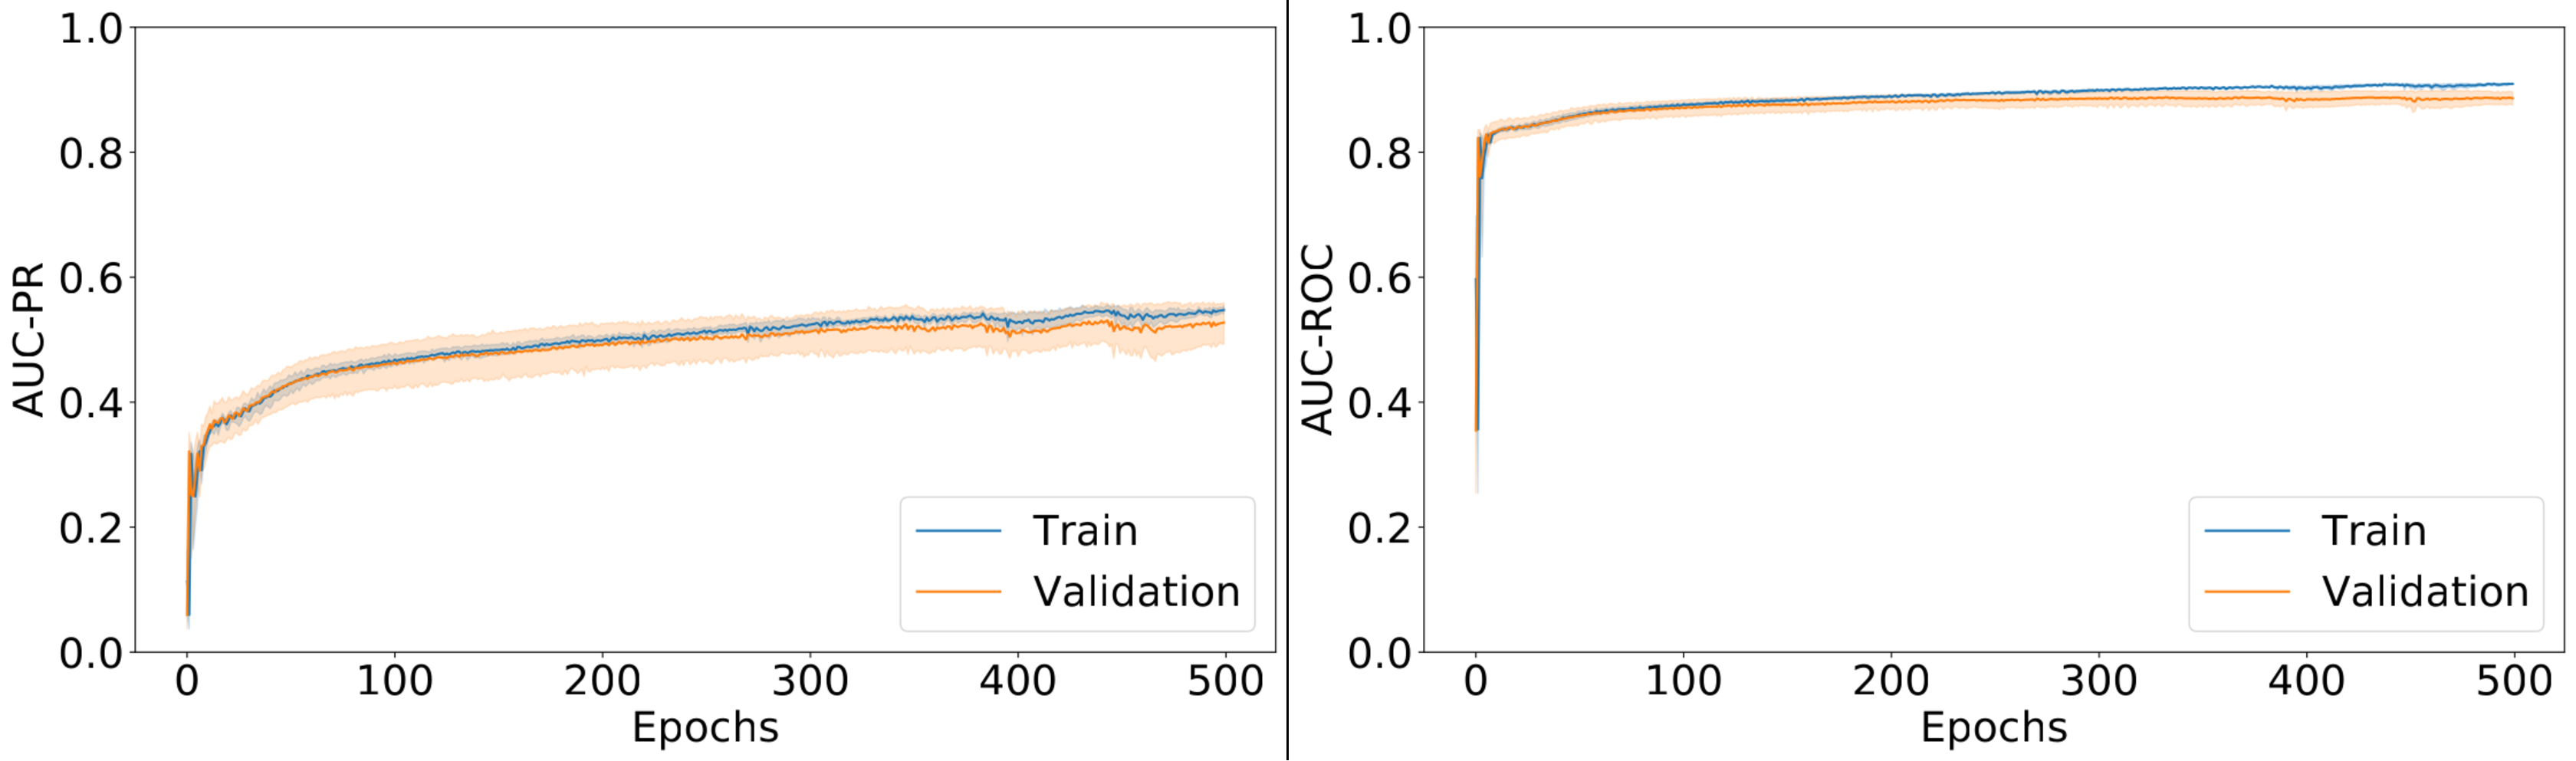
\includegraphics[width=\textwidth]{images/results/aucpr_roc_pcnet.pdf}}
\hspace{\fill}
   \subfloat[STRING \label{aucpr_roc_string}]{%
      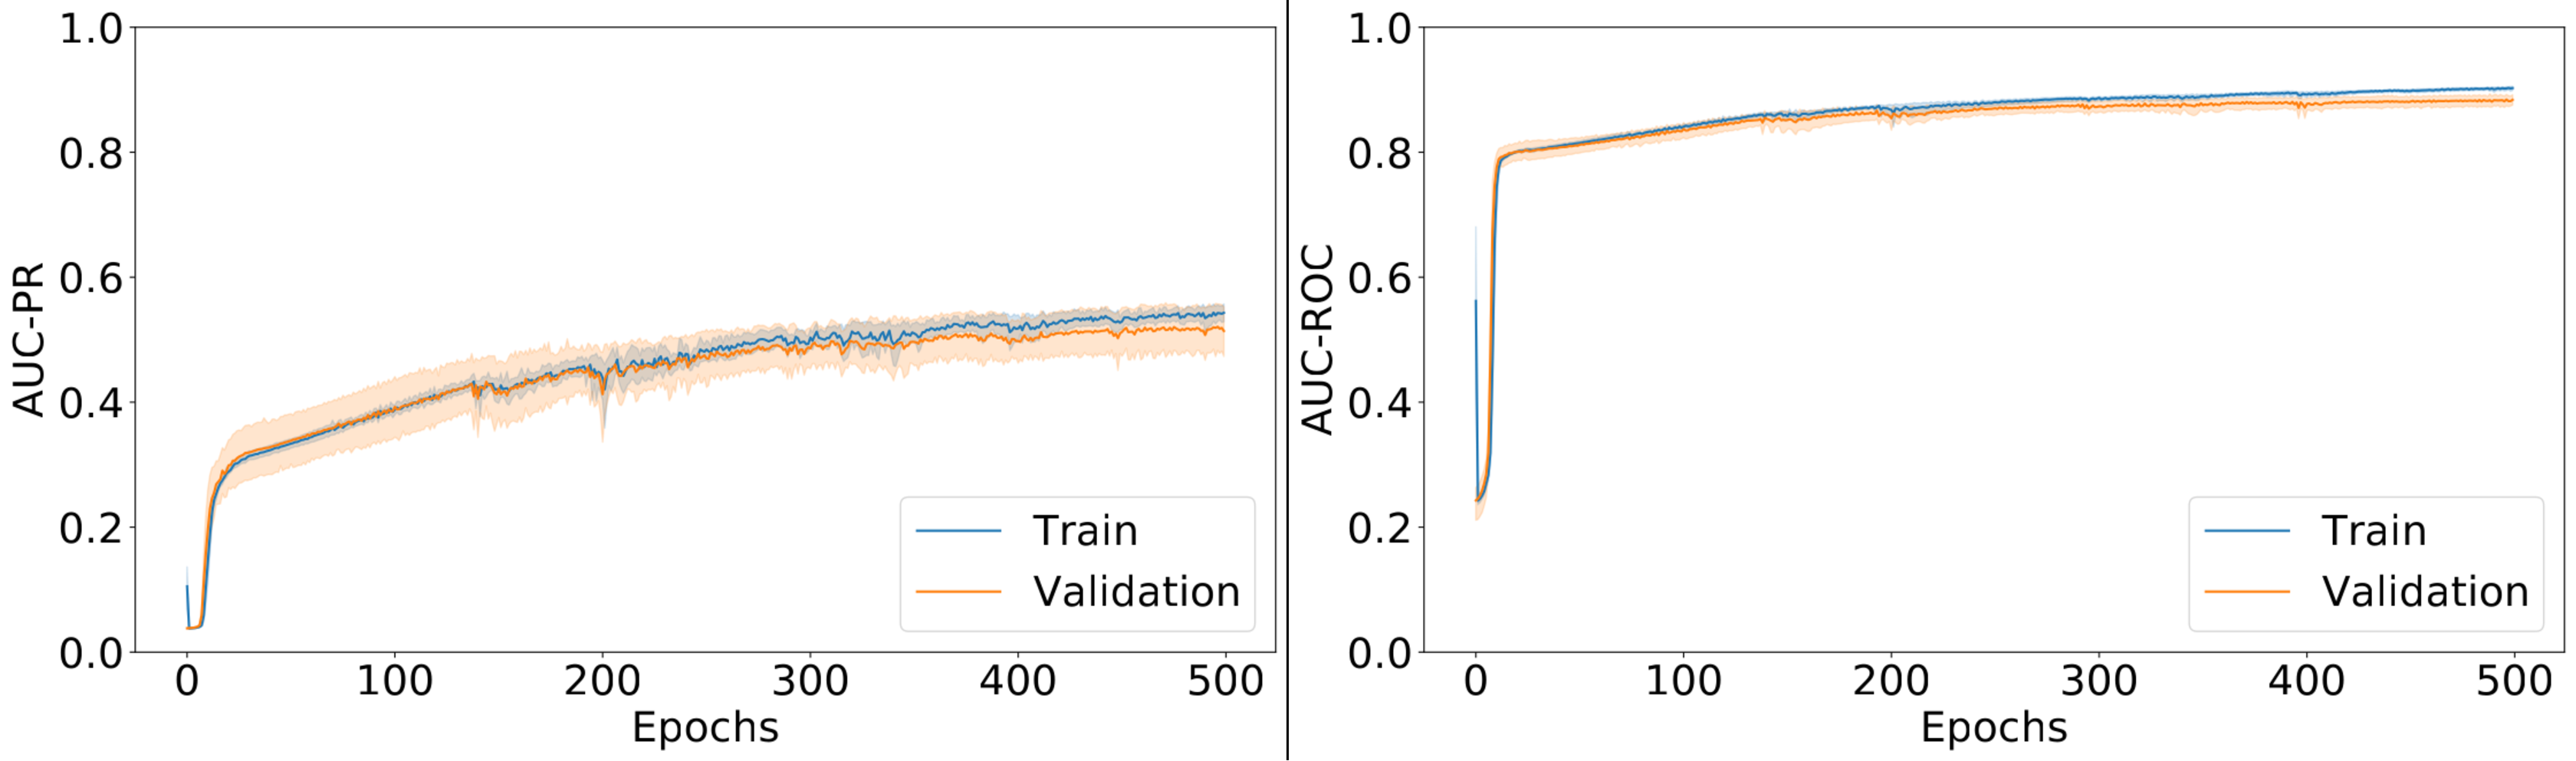
\includegraphics[width=\textwidth]{images/results/aucpr_roc_string.pdf}}\\

\label{fig:aucpr_roc_best3}
\end{figure*}

In Figure \ref{fig:aucpr_roc_best3}, we can note that in some cases, such as for MULTINET, the model shows signs of overfitting from 200 epochs onwards. This was also observed for HPRD, IREF, and CPDB (Figure~\ref{fig:aucpr_roc_worse3}). Despite this, we still noted an improvement in the performance of models for the test data, compared with the metrics without hyperparameter optimization reported in Chapter \ref{sec:results:comparative_evaluation}. We remind that the common test set used across the PPI networks, as presented in Section \ref{sec:independent_testset}, contains 1134 labeled genes: 159 positives and 975 negatives examples. 

Table \ref{tab:perform_test_set} summarizes the performance metrics for the independent test set of the GCN models trained on each of the PPI networks. AUC-PR values varied from 0.5646 for the CPDB network to 0.6358 for the STRING network. Accuracy and AUC-ROC values, as expected, are higher, reaching values above 0.80, except for the accuracy of the PCNET network. For the three smallest PPI networks, there was an increase of 10.42\%, on average, for the AUC-PR performance. 


\begin{table}[!ht]
\centering
\caption{Performance of individual GCN-based models on the test set\label{tab:perform_test_set}}
\begin{tabular}{lccc}
\hline
\multicolumn{1}{c}{PPI Network} & \multicolumn{3}{c}{Metrics}                         \\ \hline
                                & Accuracy        & AUC-ROC         & AUC-PR          \\ \cline{2-4} 
HPRD                            & 0.8889          & 0.8433          & 0.5768          \\
MULTINET                        & 0.8915          & 0.8303          & 0.5947          \\
IREF                            & 0.8827          & 0.8063          & 0.5663          \\
CPDB                            & 0.8642          & 0.8314          & 0.5646          \\
PCNET                           & 0.7795          & 0.8527          & 0.5925          \\
STRING                          & \textbf{0.8951} & \textbf{0.8798} & \textbf{0.6358} \\ \hline
\end{tabular}
\end{table}

However, even with hyperparameters optimization, the performance of the GCN-based models, in general, did not exceed an AUC-PR of 0.6, such that compared to other related works, the performance of our models are still limited.  \citet{schulte2021integration}, for example, considered the state-of-the-art among related works, reported AUC-PR values of 0.74 and 0.68 
with the GCN algorithm and the MULTINET and PCNET PPI networks, respectively. However, the authors use a different cost-sensitive loss function, distinct sets of positively and negatively labeled data, and also different data pre-processing steps -- all of which can impact the results.

In comparison to other relevant studies, we can include two cancer-specific approaches, namely MutSigCV \cite{lawrence2013mutational} and 20/20+ \cite{Tokheim2016}, which employed different networks and achieved AUCPR average results of 0.36 and 0.63, respectively. Additionally, the author of the EMOGI model \cite{schulte2021integration} proposed a baseline approach that utilizes a Random Forest and achieved an average AUCPR of 0.58 across the analyzed networks, relying only in the extracted features, as we did in Section \ref{sec:results:comparative_evaluation:rq4}.

\begin{figure*}[!ht]
    \centering
      \caption{Predicted probabilities for the test set using the STRING PPI network for training the GCN model. The red dots represent driver genes and the blue dots represent passenger genes. The confusion matrix is extracted considering a probability threshold of 0.5.}
    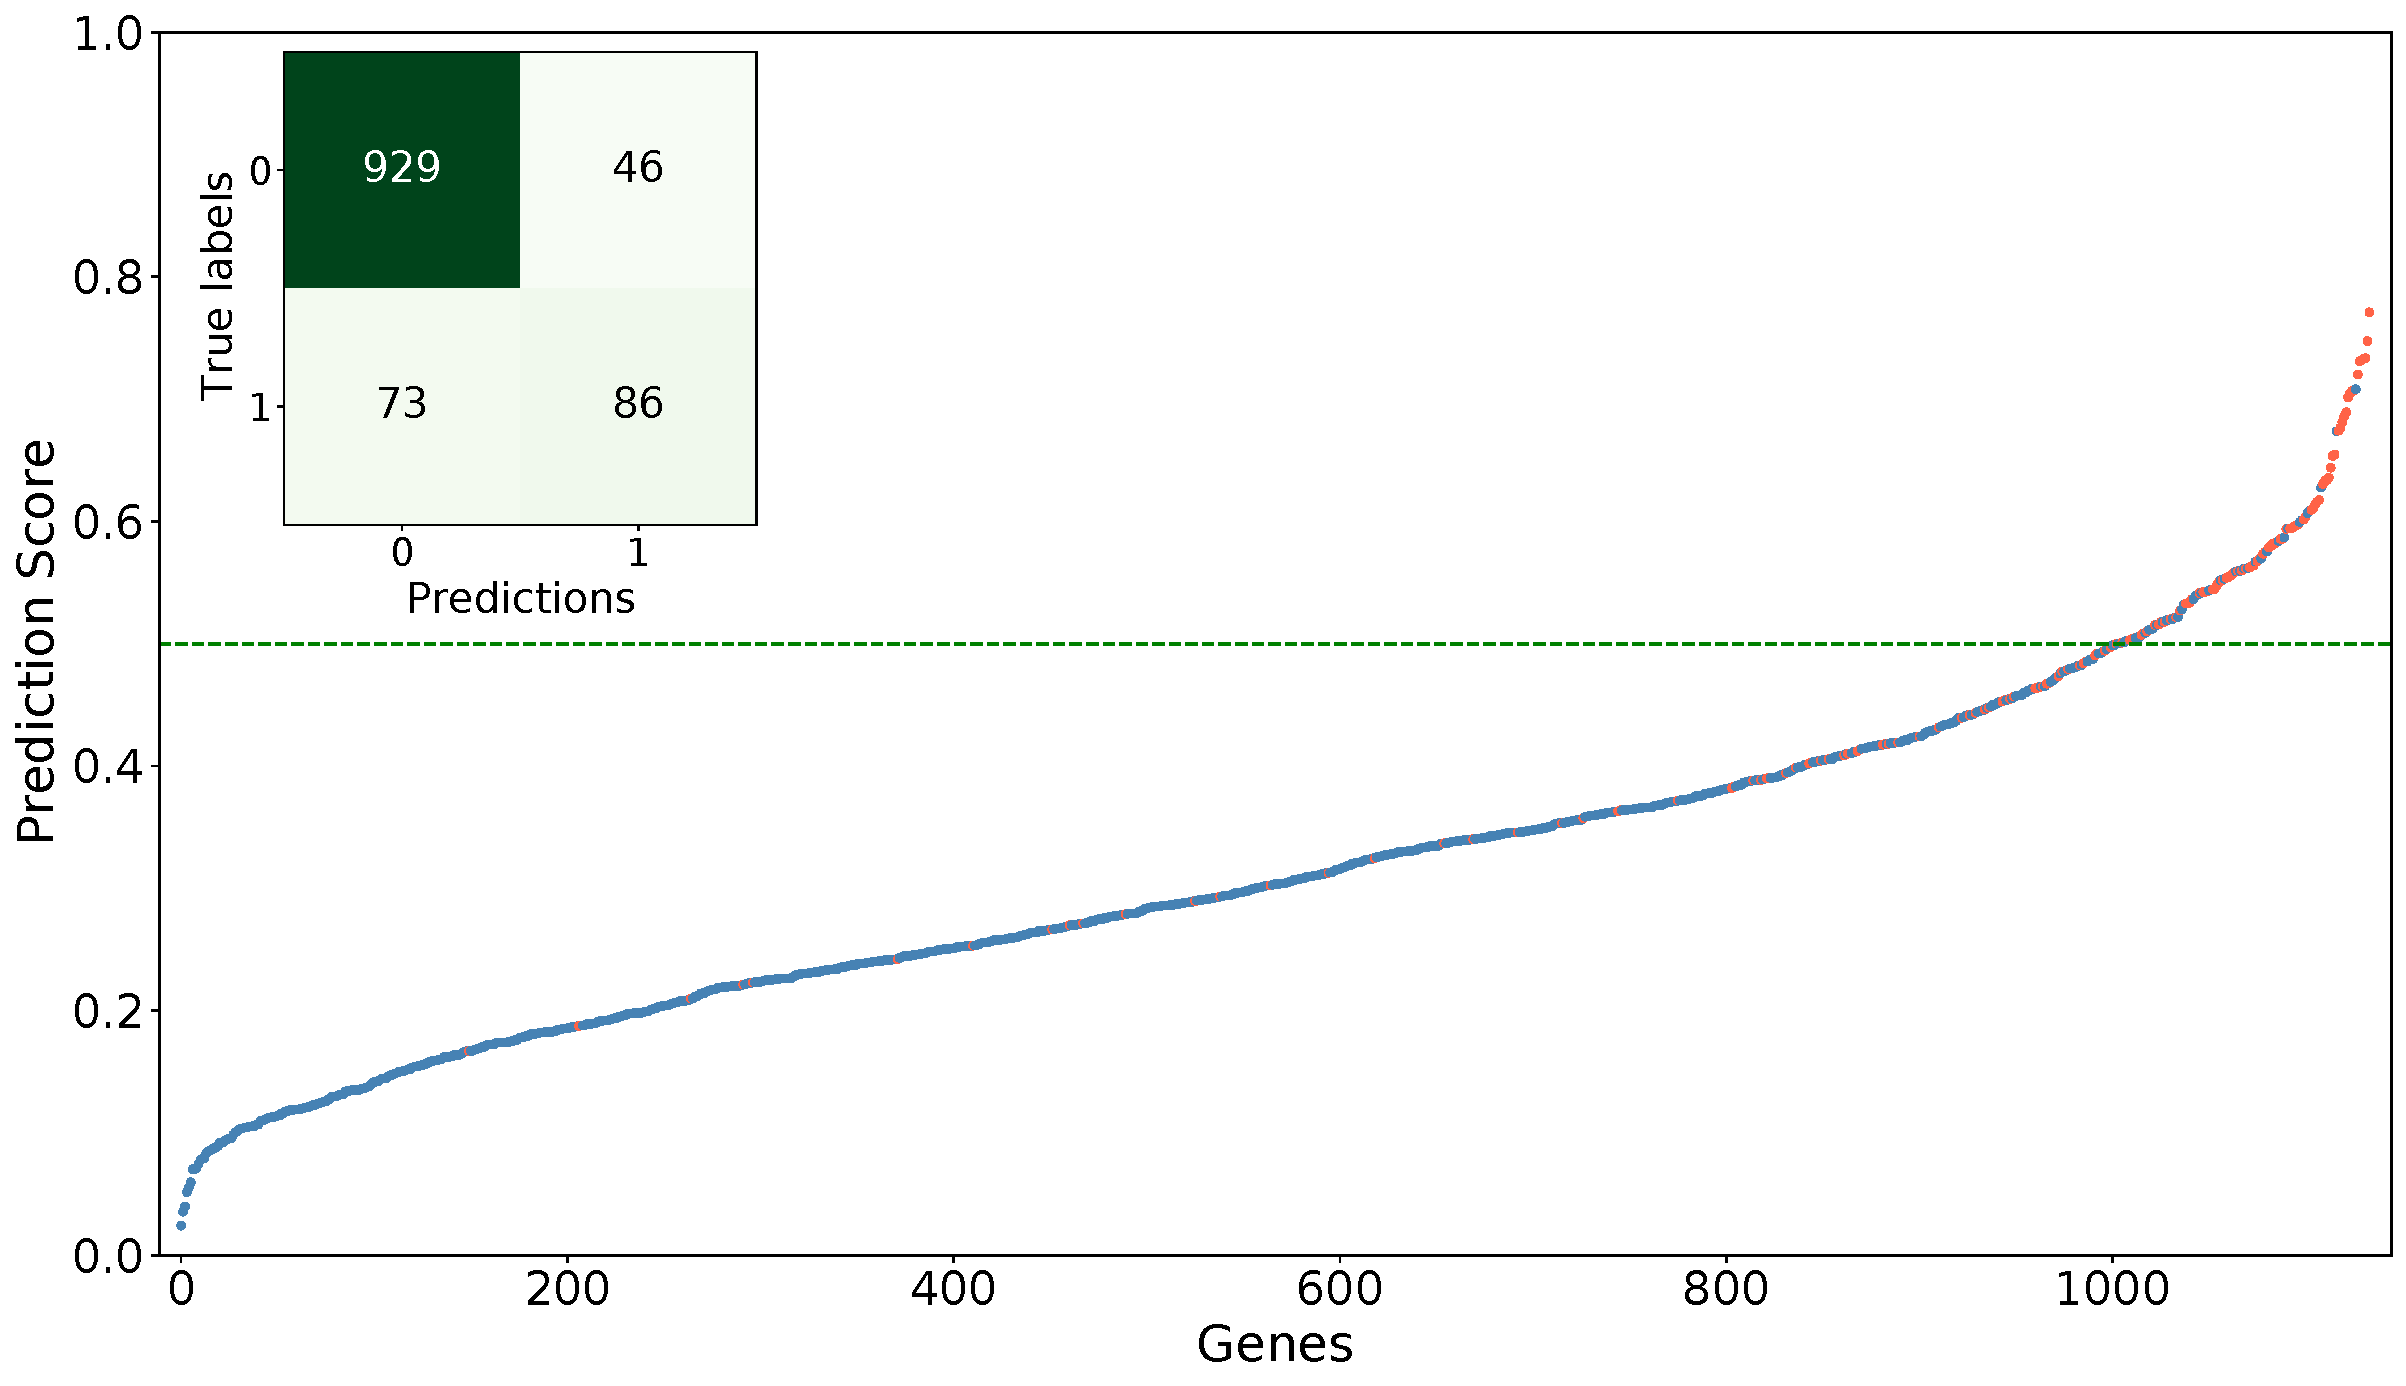
\includegraphics[width=0.9\textwidth]{images/results/test_predict_string.pdf}
    \label{fig:test_predict_string}
    \legend{Source: Prepared by the author}
\end{figure*}


Figure \ref{fig:test_predict_string} presents a scatterplot with the predicted probability (y-axis) for each gene (x-axis) in the test set using the STRING PPI network to train the GCN model. The colors indicate the true class for the gene: the red dots represent driver genes, and the blue dots represent passenger genes. The confusion matrix considering a probability threshold of 0.5 is computed and provided at the top left corner. There were a total of 132 genes predicted as drivers by the model,  86 of them correctly assigned to the positive class. 






\subsection{Predictive performance of ensemble-based prediction models for the test set}


Continuing our analysis of GCN for CDGs prediction, we investigated the collective performance of all PPI networks in the test set. Our objective is to determine whether combining multiple PPI networks can lead to superior predictions. We employed two main approaches for combining the networks: unifying the nodes and edges of the six PPI networks into a single network, which we refer to as the UNION PPI network (as explained in Section~\ref{sec:materials_methods:ppinets}), and applying aggregation methods to the outputs of six individual GCN models, each trained with a specific PPI network. The latter approach utilized ensemble learning strategies outlined in Section~\ref{sec:ensemble_training}, resulting in the Ensemble-Majority and the Ensemble-Average models.

\begin{figure*}[!b]
    \centering
      \caption{Learning curves for the UNION PPI network in terms AUC-PR and AUC-ROC.}
    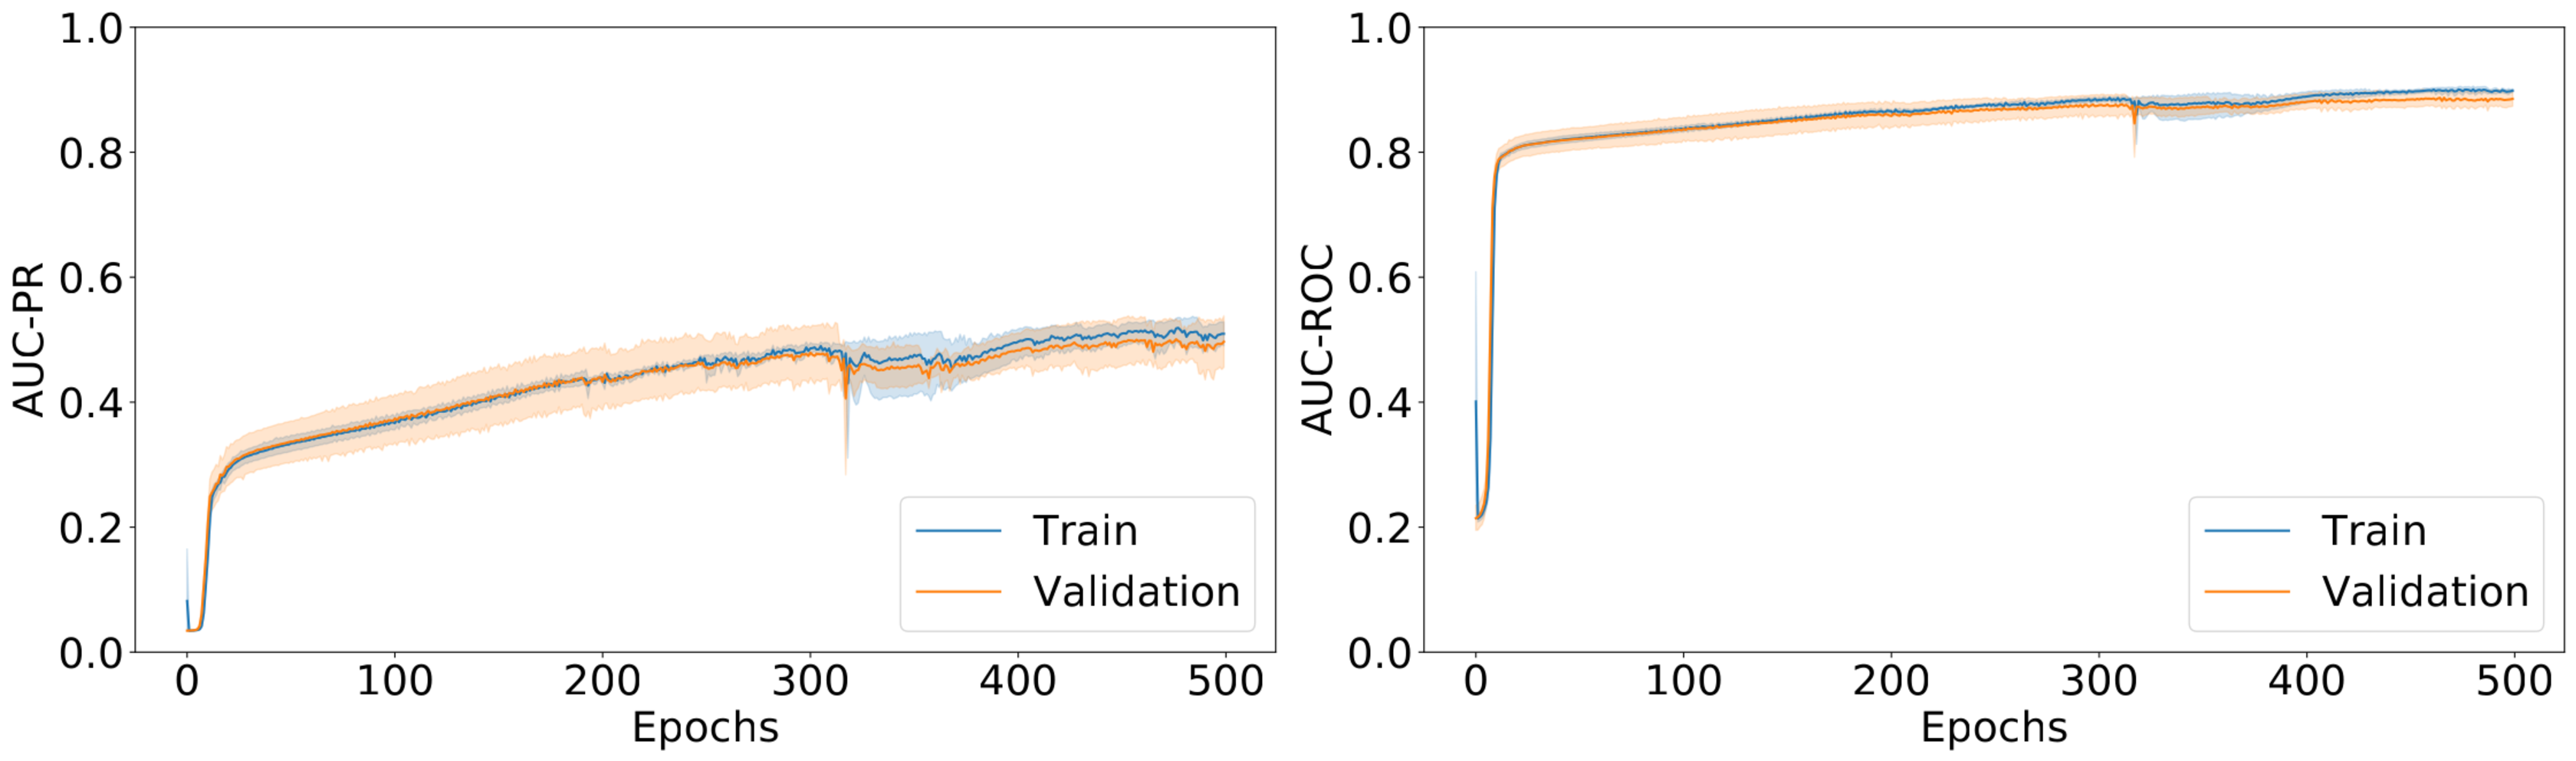
\includegraphics[width=\textwidth]{images/results/aucpr_roc_unity.pdf}
    \label{fig:aucpr_roc_unity}
\end{figure*}

We note that due to the large dimension and complexity of the UNION PPI network (\ie 7,365,082 edges and 19,602 nodes), instead of conducting a hyperparameter optimization for a GCN trained with this specific network, we used the best hyperparameters found for the STRING PPI network (\ie the largest network collected from literature). 
The training and validation performance for the UNION PPI network, shown in Figure \ref{fig:aucpr_roc_unity}, achieved marks similar to those obtained with the other networks. We obtained an average AUC-PR value of 0.4969 in the validation data, corroborating the difficulty in predicting true positives faced in our domain. The average AUC-ROC value was 0.8854, still consistent with the results obtained individually from the other networks.



\begin{figure*}[!th]
    \centering
      \caption{Predicted probabilities for the test set using the UNION PPI network for training the GCN model. The red dots represent driver genes and the blue dots represent passenger genes.  The confusion matrix is extracted considering a probability threshold of 0.5.}
    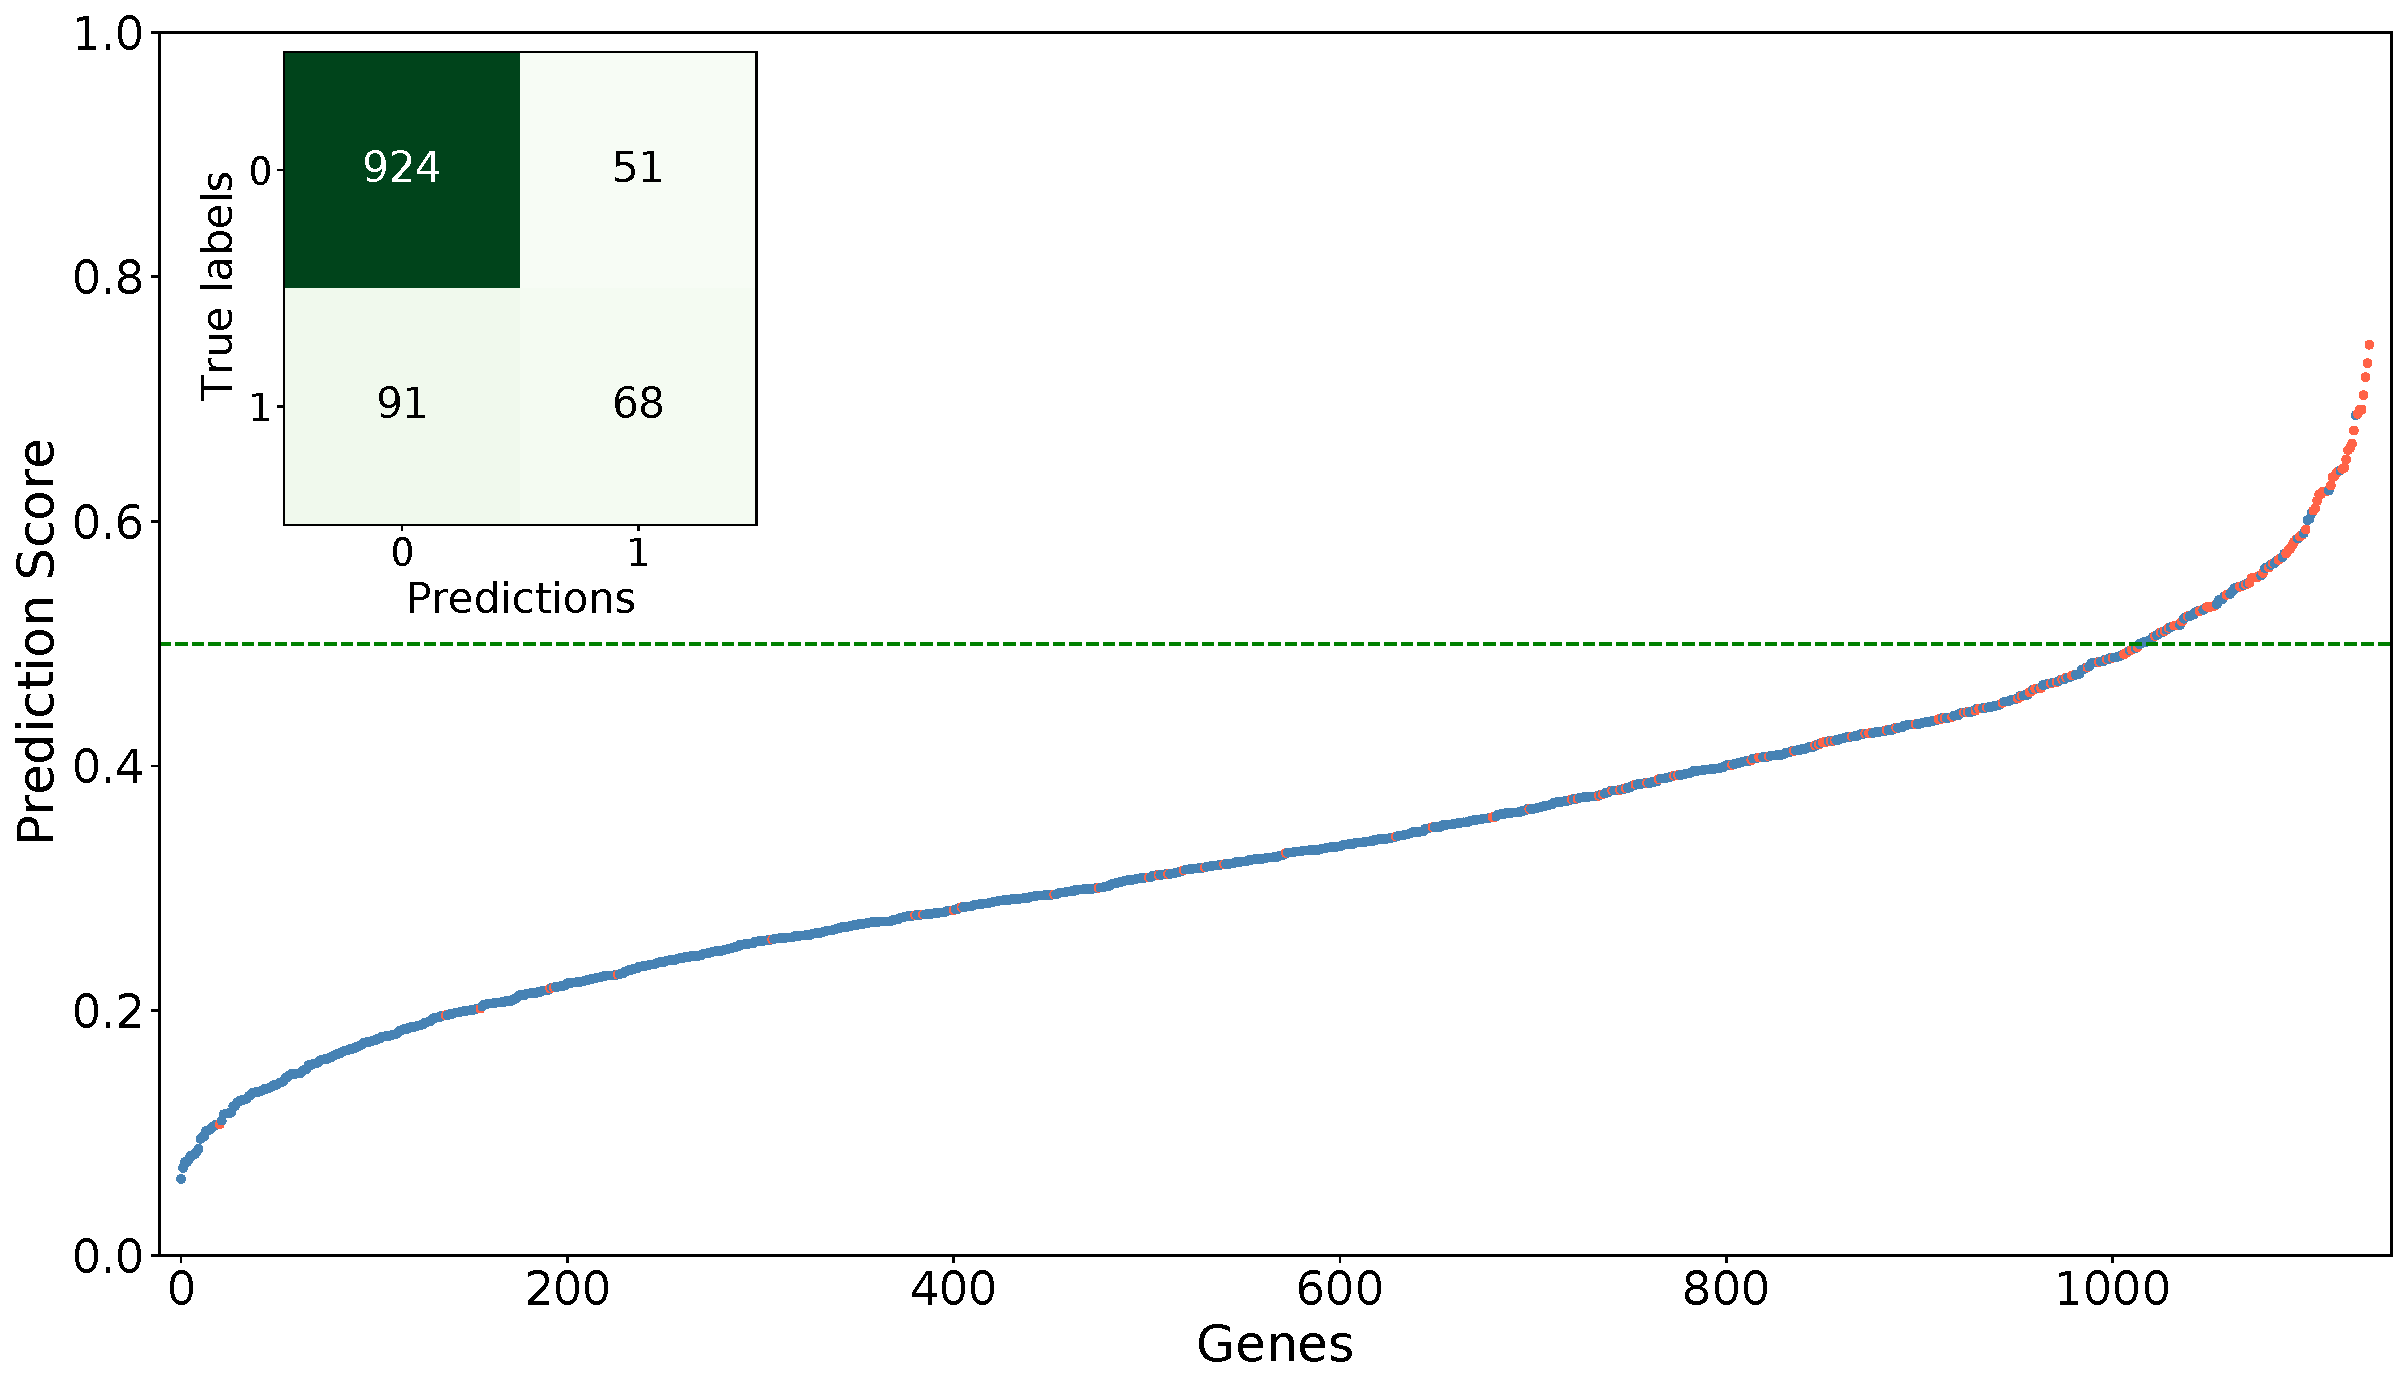
\includegraphics[width=0.9\textwidth]{images/results/test_predict_unity.pdf}
    \label{fig:test_predict_unity}
\end{figure*}

However, for the test set, we obtained an AUC-PR value of 0.5579, indicating that the simple merging of the nodes and edges of all PPI networks was not effective in improving the results compared to the individual PPI networks. Figure \ref{fig:test_predict_unity} shows the predicted probabilities for the labeled genes in the test set and also the confusion matrix for a probability threshold of 0.5. The GCN model based on the UNION PPI network predicted 119 genes as cancer drivers, where only 68 of them are true positives.

Finally, we compared another interesting approach to combining the knowledge contained in distinct PPI networks inspired by the ensemble learning paradigm. We analyzed the results for the Ensemble-Majority and Ensemble-Average. We note that while the former provides only predicted class labels due to the type of aggregation based on class votes, the latter provides predicted class labels and predicted class probabilities. 

The general performance of these models in predicting the genes of the test set is summarized in Figure \ref{fig:test_matrix_ensemble_models}. For both models, we applied the standard probability threshold of 0.5 to extract class labels. A clear impact of the two ensemble approaches, as compared to the confusion matrices shown for the STRING (Figure~\ref{fig:test_predict_string}) and the UNION (Figure~\ref{fig:test_predict_unity}) PPI networks, is the reduction in the number of false positives. The Ensemble-Majority predicted a total of 110 driver genes, from which 80 are true positives and 30 are false positives. The Ensemble-Average predicted a total of 92 driver genes, from which 73 are true positives and 19 are false positives. However, the ensemble methods failed to identify 79 and 86 drivers (\ie false negatives) at the probability threshold used.

\begin{figure*}[!ht]
\centering
\caption{Confusion matrix for the test set, analyzing the ensemble models (a) Ensemble-Majority and (b) Ensemble-Average.}

   \subfloat[Ensemble-Majority \label{fig:test_matrix_major_vot} ]{%
      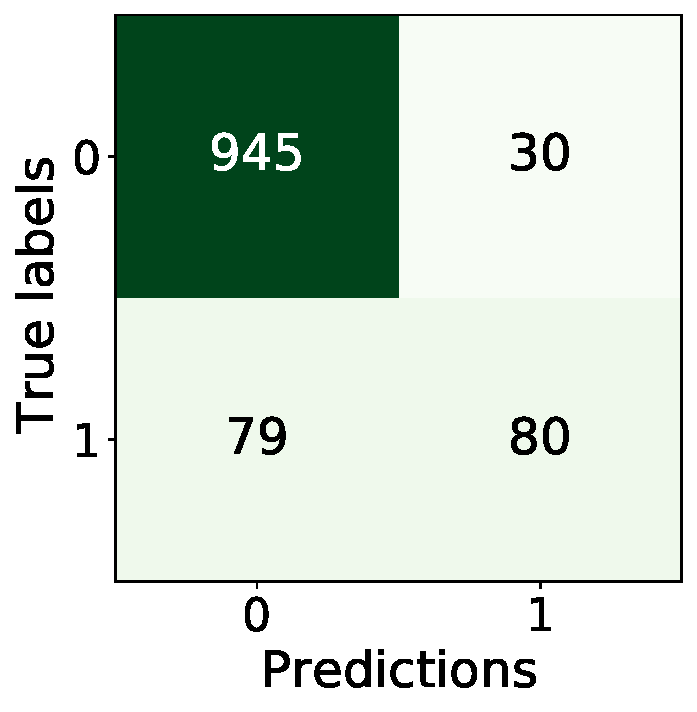
\includegraphics[width=0.35\textwidth]{images/results/test_matrix_major_vot.pdf}}
\hspace{1em}
   \subfloat[Ensemble-Average \label{fig:test_matrix_average}]{%
      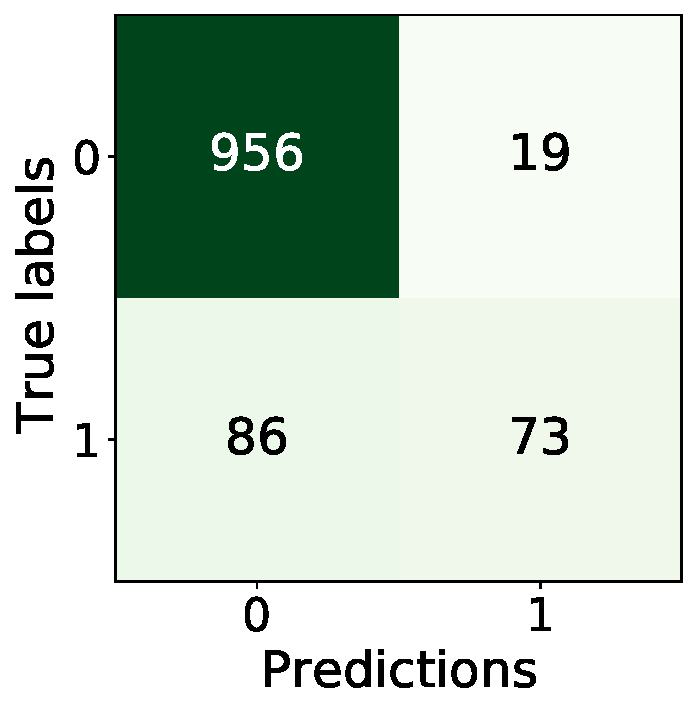
\includegraphics[width=0.35\textwidth]{images/results/test_matrix_average.pdf}}\\

\label{fig:test_matrix_ensemble_models}
\end{figure*}

We compared the predictions of individual models and ensemble-based models using a common test set. We summarized the number of predictions per class, as well as the values of TP, FP, TN, and FN from their corresponding confusion matrices. Table~\ref{tab:prediction_test_set} shows the results, with the first line displaying the reference numbers for the test set and the following lines reporting the prediction results for each discussed model. For easier comparison, we also included the precision (prec) and recall (rec) for each model.

We observed that while the IREF-based prediction model had the highest precision, its recall was very low, correctly identifying only 28 true drivers from the test set. On the other hand, the PCNET-based prediction model had the highest recall at the expense of lower precision. The Ensemble-Average model had the most balanced performance in terms of precision and recall.




\begin{table}[!bh]
\centering
\caption{Summary of models predictions for the independent test set. \label{tab:prediction_test_set}}
\resizebox{\textwidth}{!}{
\begin{tabular}{lcccccccc}
\hline
                   & \#Drivers & \#Passengers                 & \multicolumn{1}{c}{TP} & \multicolumn{1}{c}{FP} & \multicolumn{1}{c}{TN} & \multicolumn{1}{c}{FN} &  \multicolumn{1}{c}{Prec} &  \multicolumn{1}{c}{Rec}\\ \hline
Test Set           & 159    & \multicolumn{1}{c|}{975}  & -                      & -                      & -                      & -                   & -                      & -  \\
HPRD     & 85     & \multicolumn{1}{c|}{1049} & 59                     & 26                     & 949                    & 100  & 0.6941 & 0.3711                   \\
MULTINET & 74     & \multicolumn{1}{c|}{1060} & 55                     & 19                     & 956                    & 104 & 0.7432  & 0.3459                 \\
IREF     & 30     & \multicolumn{1}{c|}{1104} & 28                     & 2                      & 973                    & 131  & 0.9333 & 0.1761                   \\
CPDB     & 173    & \multicolumn{1}{c|}{961}  & 89                     & 84                     & 891                    & 70  & 0.5145 & 0.5597                   \\
PCNET    & 337    & \multicolumn{1}{c|}{797}  & 123                    & 214                    & 761                    & 36 & 0.3650 & 0.7736                    \\
STRING   & 132    & \multicolumn{1}{c|}{1002} & 86                     & 46                     & 929                    & 73   & 0.6515 & 0.5409                  \\
Predicted UNION    & 119    & \multicolumn{1}{c|}{1015} & 68                     & 51                     & 924                    & 91 & 0.5714 & 0.4277                     \\ 
Ensemble-Majority  & 110    & \multicolumn{1}{c|}{1024} & 80                     & 30                     & 945                    & 79 & 0.7273 & 0.5031                    \\
Ensemble-Average   & 92     & \multicolumn{1}{c|}{1042} & 73                     & 19                     & 956                    & 86 & 0.7935 & 0.4591                     \\
\hline
\end{tabular}}
\end{table}





Finally, we also plot the precision-recall curves (Figure~\ref{fig:aucpr_curve}) for all proposed GCN models except the Ensemble-Majority one. This model was not included in the analysis because it does not provide predicted class probabilities needed to analyze the curve. This analysis corroborates the fact that the Ensemble-Average GCN model tends to perform better than the other models in this classification task, as it presented the highest AUC-PR score (AUC-PR = 0.677).

\begin{figure*}[!th]
    \centering
      \caption{Precision-Recall curves for GCN models predictions for the test set.}
    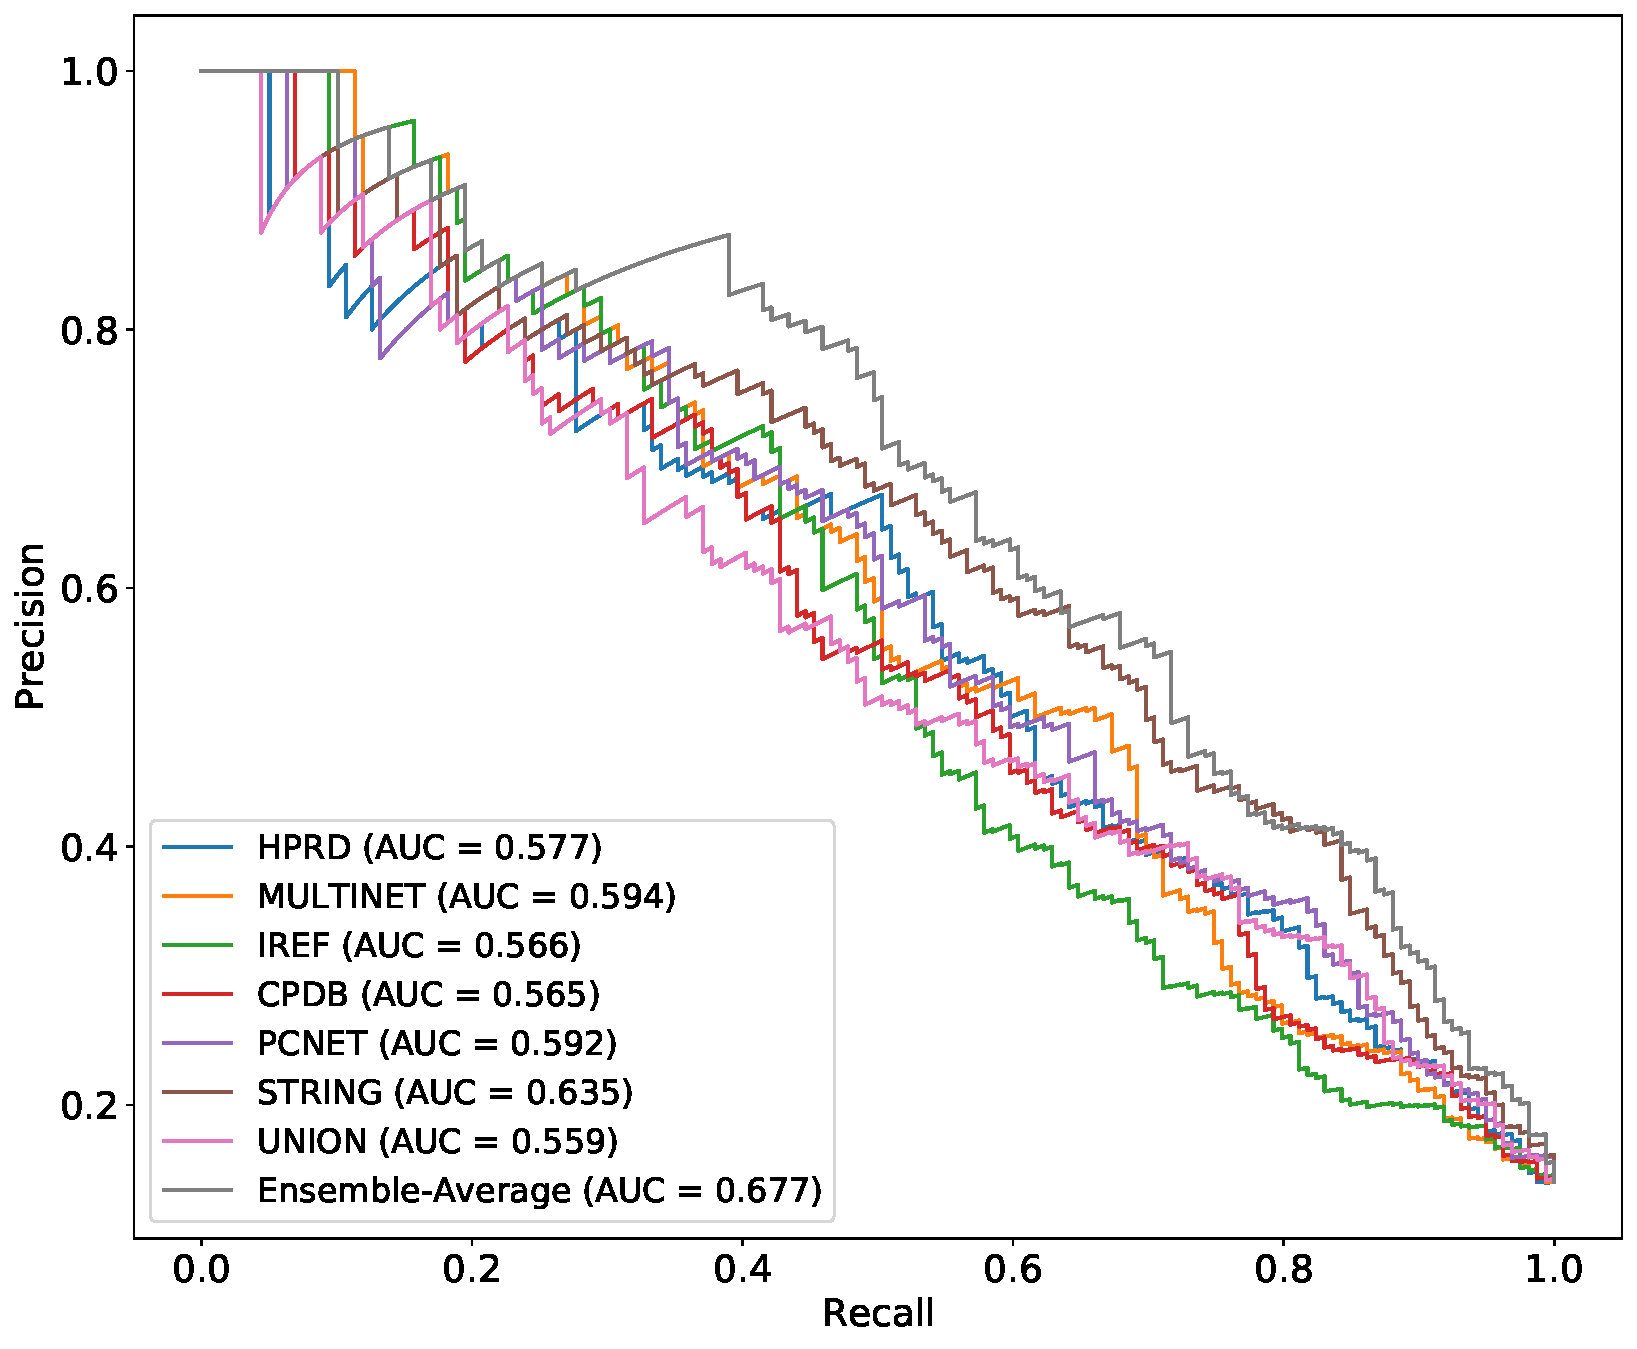
\includegraphics[width=0.9\textwidth]{images/results/aucpr_curve4.pdf}
    \label{fig:aucpr_curve}
\end{figure*}



\subsection{Analysis of GCN-based predictions for unlabelled nodes}

The main goal of our work is to develop and evaluate a GCN-based model for the prediction of CDGs. However, we are also interested in identifying potential driver genes among the unlabeled genes of the PPI networks. This could be interesting since it would enable pointing out candidate driver genes for further experimental investigation. In this section, we conduct and discuss this analysis. 

The GCN models were applied for the classification of the unlabeled nodes of their underlying PPI network (or the multiple networks, in case of the ensemble approaches). As an example, Figure \ref{fig:all_predict_string} displays a scatterplot for the predicted probabilities of all nodes in the STRING PPI network. Red dots represent true driver genes, blue dots represent true passenger genes, and gray dots represent unlabeled genes. Using a probability threshold of 0.5 represented by the green dashed line, several of the unlabeled genes are classified as cancer driver genes by our GCN model based on the STRING PPI network. The same visualization is provided for the other PPI networks in the Appendix~\ref{sec:appendix_cap6}, Figure \ref{fig:pred_samall3} and Figure~\ref{fig:pred_larger2}.



\begin{figure*}[!ht]
    \centering
      \caption{Predicted probabilities for all genes in the STRING PPI network using the trained GCN model.}
    
\includegraphics[width=0.9\textwidth]{images/testes/all_predict_string.pdf}
    \label{fig:all_predict_string}
\end{figure*}


By examining the prediction for the complete set of nodes comprised by a PPI network, we can assess the behavior of unlabeled genes that received the same predictions in different models. 
Table \ref{tab:top_candidatos} presents in the first column a subset of 10 genes that were unanimously predicted as cancer driver genes by the six GCN models trained in the PPI networks collected from the literature. The complete list of the 33 candidate cancer driver genes predicted by the six individual GCN-based models is provided in the Appendix~\ref{sec:appendix_cap6} (Table \ref{tab:lista_pred_candidates}); however, we choose to show in the Table the 10 genes with the highest predicted probabilities for the \textit{driver} class across individual models. In addition, 1477 genes were unanimously predicted as passengers by the six individual models, from which we select a sample of 33 to present in Table \ref{tab:lista_pred_candidates}, also prioritizing those with higher predicted probabilities.


\begin{table}[!ht]
\centering
\caption{Top ten candidate driver genes with the highest predicted probabilities according to some selected approaches.\label{tab:top_candidatos}}
\begin{tabular}{ccc}
\hline
\begin{tabular}[c]{@{}c@{}}Predicted by models \\ for the six PPI networks\end{tabular} & \begin{tabular}[c]{@{}c@{}}Predicted by model \\ for the UNION network\end{tabular} & \begin{tabular}[c]{@{}c@{}}Predicted by the \\ Ensemble-Average model\end{tabular} \\ \hline
HDAC2                                                                    & ALB                                                                   & GRB2                                                               \\
\textbf{SP1}                                                             & APP                                                                   & HDAC2                                                              \\
PTK2                                                                     & ELAVL1                                                                & HDAC3                                                              \\
HDAC3                                                                    & ETS1                                                                  & KAT2B                                                              \\
UBE2I                                                                    & FOS                                                                   & NR3C1                                                              \\
NR3C1                                                                    & GAPDH                                                                 & PRKCA                                                              \\
CDK1                                                                     & NFKB1                                                                 & PTK2                                                               \\
KAT2B                                                                    & \textbf{SP1}                                                          & RELA                                                               \\
NCK1                                                                     & TBP                                                                   & SHC1                                                               \\
PRKCA                                                                    & TCF4                                                                  & \textbf{SP1}                                                       \\ \hline
\end{tabular}
\end{table}

Table~\ref{tab:top_candidatos} also includes the top ten genes according to the probabilities for the \textit{driver} class predicted by the UNION-based GCN model and the Ensemble-Average GCN model. Six genes are present in both the unanimous predictions among individual models (first column) and in top 10 predictions for the Ensemble-Average model (third column). Only one gene, SP1 (Sp1 Transcription Factor), is predicted as candidate in all three cases analyzed in the table. Further investigation of these genes may elucidate new drivers of tumorigenesis.


Another analysis we carried out was to investigate false positives indicated with high probabilities as CDG by the proposed models. We include similarobservations as in Table~\ref{tab:top_candidatos}, but now considering false positive genes instead of candidates genes (Table~\ref{tab:top_falsos_positivos}). The first column represents genes that are originally labeled as negative genes and that were predicted as positive by five or more different networks, considering the highest probability in all networks. Only three genes were unanimously predicted as false positives for this case YWHAZ, SPTBN1 and H2BC21. The second and third column represent the original negative genes predicted as CDGs with the highest probability considering the UNION network model and the Ensemble-Average method, respectively.


\begin{table}[!ht]
\centering
\caption{Top ten false positives driver genes with the highest predicted probabilities according to some selected approaches.\label{tab:top_falsos_positivos}}
\resizebox{\textwidth}{!}{
\begin{tabular}{ccc}
\hline
\begin{tabular}[c]{@{}c@{}}False positive predicted by \\ separated models of PPI networks\end{tabular} &
  \begin{tabular}[c]{@{}c@{}}False positives predicted by \\ model for the UNION network\end{tabular} &
  \begin{tabular}[c]{@{}c@{}}False positives predicted by \\ the Ensemble-Average model\end{tabular} \\ \hline
SUMO2   & MYH14   & \textbf{YWHAZ}   \\
H2BC21  & VCAM1   & YWHAG   \\
SUMO3   & PI3     & SFN     \\
YWHAQ   & TF      & YWHAH   \\
SPTBN1  & UTRN    & SRF     \\
YWHAG   & MAFF    & IRAK1   \\
PTPRF   & SST     & MBP     \\
SRF     & \textbf{YWHAZ}   & PIN1    \\
KHDRBS1 & SMARCA5 & SMARCA5 \\
\textbf{YWHAZ}   & MBP     & PPFIA1  \\ \hline
\end{tabular}}
\end{table}


Observing the high-confidence false positives predictions of our models, we may extract insights about genes that have strong indication of involvement with cancer, perhaps as a CDG, but that were not experimentally verified as drivers of carcinogenesis. This is the case for gene YWHAZ, which was unanimously predicted as a driver by all analyzed networks, as well as by the UNION network and the Ensemble-Average model. Interestingly, prior works have discussed that YWHAZ is frequently up-regulated in multiple types of cancers and may act as an oncogene by promoting malignant properties of cancer cells \cite{gan2020role}. Thus, further investigation of false positives associated with high CDG probability is interesting to review original annotations and expand the current knowledge about CDGs.











\section{Summary}

With the best GNN algorithm selected in the previous chapter, in this chapter we seek to optimize the prediction results of the GCN model, we perform a search for better combinations of hyperparameters in each of the selected networks, to meet the different particularities of each one of them.

With this, we identified a set of genes common to all networks that could be used as test data. We then apply a new training round to each of the networks, with the optimal parameters found and with a common test set, from this we can analyze the prediction tendency of each of the networks separately by looking at this fixed list that is evaluated in the same way for all networks.

We implemented a majority voting system and utilized the average prediction scores of the networks to identify genes that were highly likely to be classified as driver genes. In addition, we devised a new network architecture by combining the nodes and edges of all six networks and removing duplicate gene links. This new network was also subjected to prediction analysis using the same ensemble, but was found to be less effective in terms of metrics than the initial ensemble network analysis.

Despite this, we successfully identified a list of candidate genes that were not previously classified as drivers or passengers but were classified as drivers in different contexts. We also identified a list of 33 candidate genes that were unanimously predicted by all selected networks to be cancer driver genes.

